\documentclass{book}
\usepackage[a4paper,top=2.5cm,bottom=2.5cm,left=2.5cm,right=2.5cm]{geometry}
\usepackage{makeidx}
\usepackage{natbib}
\usepackage{graphicx}
\usepackage{multicol}
\usepackage{float}
\usepackage{listings}
\usepackage{color}
\usepackage{ifthen}
\usepackage[table]{xcolor}
\usepackage{textcomp}
\usepackage{alltt}
\usepackage{ifpdf}
\ifpdf
\usepackage[pdftex,
            pagebackref=true,
            colorlinks=true,
            linkcolor=blue,
            unicode
           ]{hyperref}
\else
\usepackage[ps2pdf,
            pagebackref=true,
            colorlinks=true,
            linkcolor=blue,
            unicode
           ]{hyperref}
\usepackage{pspicture}
\fi
\usepackage[utf8]{inputenc}
\usepackage[french]{babel}

\usepackage{mathptmx}
\usepackage[scaled=.90]{helvet}
\usepackage{courier}
\usepackage{sectsty}
\usepackage{amssymb}
\usepackage[titles]{tocloft}
\usepackage{doxygen}
\lstset{language=C++,inputencoding=utf8,basicstyle=\footnotesize,breaklines=true,breakatwhitespace=true,tabsize=8,numbers=left }
\makeindex
\setcounter{tocdepth}{3}
\renewcommand{\footrulewidth}{0.4pt}
\renewcommand{\familydefault}{\sfdefault}
\hfuzz=15pt
\setlength{\emergencystretch}{15pt}
\hbadness=750
\tolerance=750
\begin{document}
\hypersetup{pageanchor=false,citecolor=blue}
\begin{titlepage}
\vspace*{7cm}
\begin{center}
{\Large Algorithms Frame\-Work \\[1ex]\large 1.\-0 }\\
\vspace*{1cm}
{\large Généré par Doxygen 1.8.1.2}\\
\vspace*{0.5cm}
{\small Dimanche Janvier 20 2013 14:24:32}\\
\end{center}
\end{titlepage}
\clearemptydoublepage
\pagenumbering{roman}
\tableofcontents
\clearemptydoublepage
\pagenumbering{arabic}
\hypersetup{pageanchor=true,citecolor=blue}
\chapter{Algorithms Frame\-Work}
\label{index}\hypertarget{index}{}Il s'agit d'un ensemble de classes, modèles de classes, fonctions, modèles de fonctions, etc. permettant d’écrire des algorithmes et d’effectuer des mesures sur leurs exécutions. L’utilisateur de ce canevas pourra par exemple être simplement conduit à indiquer qu’il souhaite mesurer un algorithme sur des Entiers (exemple quicksort sur les tableaux d’ints).

\begin{DoxyAuthor}{Auteur}
Richard Isabelle, Abou Haydar Elias, Ourfahli Anthony 
\end{DoxyAuthor}

\chapter{Index des classes}
\section{Hiérarchie des classes}
Cette liste d'héritage est classée approximativement par ordre alphabétique \-:\begin{DoxyCompactList}
\item \contentsline{section}{Object$<$ O, stat $>$}{\pageref{class_object}}{}
\item \contentsline{section}{Object$<$ float, stat $>$}{\pageref{class_object}}{}
\begin{DoxyCompactList}
\item \contentsline{section}{Float$<$ stat $>$}{\pageref{class_float}}{}
\end{DoxyCompactList}
\item \contentsline{section}{Object$<$ int, stat $>$}{\pageref{class_object}}{}
\begin{DoxyCompactList}
\item \contentsline{section}{Entier$<$ stat $>$}{\pageref{class_entier}}{}
\end{DoxyCompactList}
\item \contentsline{section}{Object$<$ string, stat $>$}{\pageref{class_object}}{}
\begin{DoxyCompactList}
\item \contentsline{section}{String$<$ stat $>$}{\pageref{class_string}}{}
\end{DoxyCompactList}
\item \contentsline{section}{Stat}{\pageref{class_stat}}{}
\end{DoxyCompactList}

\chapter{Index des classes}
\section{Liste des classes}
Liste des classes, structures, unions et interfaces avec une brève description \-:\begin{DoxyCompactList}
\item\contentsline{section}{\hyperlink{class_entier}{Entier$<$ stat $>$} }{\pageref{class_entier}}{}
\item\contentsline{section}{\hyperlink{class_float}{Float$<$ stat $>$} }{\pageref{class_float}}{}
\item\contentsline{section}{\hyperlink{class_object}{Object$<$ O, stat $>$} }{\pageref{class_object}}{}
\item\contentsline{section}{\hyperlink{class_stat}{Stat} }{\pageref{class_stat}}{}
\item\contentsline{section}{\hyperlink{class_string}{String$<$ stat $>$} }{\pageref{class_string}}{}
\end{DoxyCompactList}

\chapter{Documentation des classes}
\hypertarget{class_entier}{\section{Référence du modèle de la classe Entier$<$ stat $>$}
\label{class_entier}\index{Entier$<$ stat $>$@{Entier$<$ stat $>$}}
}


{\ttfamily \#include $<$Entier.\-hpp$>$}



Graphe d'héritage de Entier$<$ stat $>$\-:\nopagebreak
\begin{figure}[H]
\begin{center}
\leavevmode
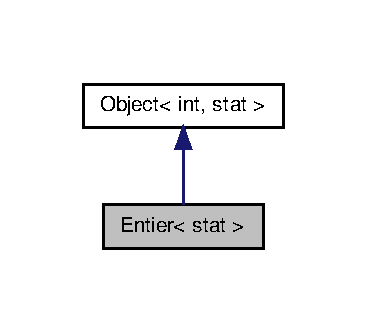
\includegraphics[width=176pt]{class_entier__inherit__graph}
\end{center}
\end{figure}


Graphe de collaboration de Entier$<$ stat $>$\-:\nopagebreak
\begin{figure}[H]
\begin{center}
\leavevmode
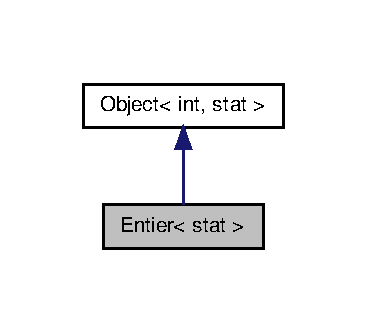
\includegraphics[width=176pt]{class_entier__coll__graph}
\end{center}
\end{figure}
\subsection*{Fonctions membres publiques}
\begin{DoxyCompactItemize}
\item 
\hyperlink{class_entier_a1e2d7505c454b85ef1201dd48b794812}{Entier} ()
\item 
\hyperlink{class_entier_aeb4c79c0bcc38ccc9c5a1ad043803b2b}{Entier} (const int \&i)
\item 
virtual \hyperlink{class_entier_af31cb8d422ea697a4e0209bb901272ad}{$\sim$\-Entier} ()
\item 
\hyperlink{class_entier}{Entier} \hyperlink{class_entier_a3fbb1809ad562b0008ab2352a15099a6}{operator+} (const int \&i)
\item 
\hyperlink{class_entier}{Entier} \hyperlink{class_entier_a8282ad9ab4575ab6b9133b0cb1735937}{operator+} (const \hyperlink{class_entier}{Entier} \&e)
\item 
\hyperlink{class_entier}{Entier} \hyperlink{class_entier_aced3c660e95f5986b5332f35dab8c582}{operator-\/} (const int \&i)
\item 
\hyperlink{class_entier}{Entier} \hyperlink{class_entier_adac2059d0b47ad800e6720472f2e3bfe}{operator-\/} (const \hyperlink{class_entier}{Entier} \&e)
\item 
\hyperlink{class_entier}{Entier} \hyperlink{class_entier_a256b2fe208f9213b4de99c028354eb58}{operator$\ast$} (const int \&i)
\item 
\hyperlink{class_entier}{Entier} \hyperlink{class_entier_aaf553e13bb7888e9ab67744bdfce7839}{operator$\ast$} (const \hyperlink{class_entier}{Entier} \&e)
\item 
\hyperlink{class_entier}{Entier} \hyperlink{class_entier_a1aeb57f0c3b07a045f5f51d7d581efb9}{operator/} (const int \&i)
\item 
\hyperlink{class_entier}{Entier} \hyperlink{class_entier_a08f1ccbb12ca08e195c7cf98e9d749bd}{operator/} (const \hyperlink{class_entier}{Entier} \&e)
\item 
\hyperlink{class_entier}{Entier} \hyperlink{class_entier_a9a8ee8f74ab48a1eff0495788e811b68}{operator\%} (const int \&i)
\item 
\hyperlink{class_entier}{Entier} \hyperlink{class_entier_a634aaf924535952927e4a37a32f43be4}{operator\%} (const \hyperlink{class_entier}{Entier} \&e)
\item 
\hyperlink{class_entier}{Entier} \& \hyperlink{class_entier_a755888e1158fa05b5abb52b77d3b0b7d}{operator++} ()
\item 
void \hyperlink{class_entier_aab83e1feb6a831985798dc29eafd6c4f}{operator++} (int i)
\item 
\hyperlink{class_entier}{Entier} \& \hyperlink{class_entier_ac54e5be59891760a29654c65f73740bd}{operator-\/-\/} ()
\item 
void \hyperlink{class_entier_a74a16719c1cfa70aae23289076e11603}{operator-\/-\/} (int i)
\item 
\hyperlink{class_entier}{Entier} \& \hyperlink{class_entier_a9fc7f0a86ca6c2c6d1f27c46aa4091a8}{operator+=} (const int \&i)
\item 
\hyperlink{class_entier}{Entier} \& \hyperlink{class_entier_a82de36cd5797697254f0e560f3fcb749}{operator+=} (const \hyperlink{class_entier}{Entier} \&e)
\item 
\hyperlink{class_entier}{Entier} \& \hyperlink{class_entier_a2fd722ed526998dd47f37d7f1c8e973a}{operator-\/=} (const int \&i)
\item 
\hyperlink{class_entier}{Entier} \& \hyperlink{class_entier_a054bed73fefc9262c480f925cd05e53e}{operator-\/=} (const \hyperlink{class_entier}{Entier} \&e)
\item 
\hyperlink{class_entier}{Entier} \& \hyperlink{class_entier_abccfd189f2404d19598045ab77626064}{operator$\ast$=} (const int \&i)
\item 
\hyperlink{class_entier}{Entier} \& \hyperlink{class_entier_a5b18e321fd792feb1868352c12fe5ba8}{operator$\ast$=} (const \hyperlink{class_entier}{Entier} \&e)
\item 
\hyperlink{class_entier}{Entier} \& \hyperlink{class_entier_aa11ea29bf56ca06bdef29ea611016f84}{operator/=} (const int \&i)
\item 
\hyperlink{class_entier}{Entier} \& \hyperlink{class_entier_a9273b726a0f5640b4e2940e71965a4c7}{operator/=} (const \hyperlink{class_entier}{Entier} \&e)
\item 
\hyperlink{class_entier}{Entier} \& \hyperlink{class_entier_a00ae0c4500fc317f70e3bcbe8962202e}{operator\%=} (const int \&i)
\item 
\hyperlink{class_entier}{Entier} \& \hyperlink{class_entier_aa40a5ac0715408ac63d30a18e9eb66f2}{operator\%=} (const \hyperlink{class_entier}{Entier} \&e)
\end{DoxyCompactItemize}
\subsection*{Additional Inherited Members}


\subsection{Description détaillée}
\subsubsection*{template$<$Stat $\ast$ stat$>$class Entier$<$ stat $>$}

La classe \hyperlink{class_entier}{Entier} répresente un modele de classe de type int et une réference vers une instance de statistique. La classe \hyperlink{class_entier}{Entier} hérite de la spécification de \hyperlink{class_object}{Object$<$int,stat$>$} 

\subsection{Documentation des constructeurs et destructeur}
\hypertarget{class_entier_a1e2d7505c454b85ef1201dd48b794812}{\index{Entier@{Entier}!Entier@{Entier}}
\index{Entier@{Entier}!Entier@{Entier}}
\subsubsection[{Entier}]{\setlength{\rightskip}{0pt plus 5cm}template$<$Stat $\ast$ stat$>$ {\bf Entier}$<$ stat $>$\-::{\bf Entier} (
\begin{DoxyParamCaption}
{}
\end{DoxyParamCaption}
)\hspace{0.3cm}{\ttfamily [inline]}}}\label{class_entier_a1e2d7505c454b85ef1201dd48b794812}
Constructeur. Donne une valeur par défaut à un entier. 
\begin{DoxyTemplParams}{Template Parameters}
{\em stat} & réference vers la statistiques en cours d'utilisation. \\
\hline
\end{DoxyTemplParams}
\hypertarget{class_entier_aeb4c79c0bcc38ccc9c5a1ad043803b2b}{\index{Entier@{Entier}!Entier@{Entier}}
\index{Entier@{Entier}!Entier@{Entier}}
\subsubsection[{Entier}]{\setlength{\rightskip}{0pt plus 5cm}template$<$Stat $\ast$ stat$>$ {\bf Entier}$<$ stat $>$\-::{\bf Entier} (
\begin{DoxyParamCaption}
\item[{const int \&}]{i}
\end{DoxyParamCaption}
)\hspace{0.3cm}{\ttfamily [inline]}}}\label{class_entier_aeb4c79c0bcc38ccc9c5a1ad043803b2b}
Constructeur. Donne une réference vers un element de type O à cet objet. 
\begin{DoxyTemplParams}{Template Parameters}
{\em stat} & réference vers la statistiques en cours d'utilisation. \\
\hline
\end{DoxyTemplParams}

\begin{DoxyParams}{Paramètres}
{\em i} & réference vers un entier. \\
\hline
\end{DoxyParams}
\hypertarget{class_entier_af31cb8d422ea697a4e0209bb901272ad}{\index{Entier@{Entier}!$\sim$\-Entier@{$\sim$\-Entier}}
\index{$\sim$\-Entier@{$\sim$\-Entier}!Entier@{Entier}}
\subsubsection[{$\sim$\-Entier}]{\setlength{\rightskip}{0pt plus 5cm}template$<$Stat $\ast$ stat$>$ virtual {\bf Entier}$<$ stat $>$\-::$\sim${\bf Entier} (
\begin{DoxyParamCaption}
{}
\end{DoxyParamCaption}
)\hspace{0.3cm}{\ttfamily [inline]}, {\ttfamily [virtual]}}}\label{class_entier_af31cb8d422ea697a4e0209bb901272ad}
Destructeur Detruit l'objet de type \hyperlink{class_entier}{Entier} 

\subsection{Documentation des fonctions membres}
\hypertarget{class_entier_a9a8ee8f74ab48a1eff0495788e811b68}{\index{Entier@{Entier}!operator\%@{operator\%}}
\index{operator\%@{operator\%}!Entier@{Entier}}
\subsubsection[{operator\%}]{\setlength{\rightskip}{0pt plus 5cm}template$<$Stat $\ast$ stat$>$ {\bf Entier} {\bf Entier}$<$ stat $>$\-::operator\% (
\begin{DoxyParamCaption}
\item[{const int \&}]{i}
\end{DoxyParamCaption}
)\hspace{0.3cm}{\ttfamily [inline]}}}\label{class_entier_a9a8ee8f74ab48a1eff0495788e811b68}
Surcharge de l'operateur \% 
\begin{DoxyParams}{Paramètres}
{\em i} & un entier. \\
\hline
\end{DoxyParams}
\hypertarget{class_entier_a634aaf924535952927e4a37a32f43be4}{\index{Entier@{Entier}!operator\%@{operator\%}}
\index{operator\%@{operator\%}!Entier@{Entier}}
\subsubsection[{operator\%}]{\setlength{\rightskip}{0pt plus 5cm}template$<$Stat $\ast$ stat$>$ {\bf Entier} {\bf Entier}$<$ stat $>$\-::operator\% (
\begin{DoxyParamCaption}
\item[{const {\bf Entier}$<$ stat $>$ \&}]{e}
\end{DoxyParamCaption}
)\hspace{0.3cm}{\ttfamily [inline]}}}\label{class_entier_a634aaf924535952927e4a37a32f43be4}
Surcharge de l'operateur \% 
\begin{DoxyParams}{Paramètres}
{\em e} & un objet \hyperlink{class_entier}{Entier}. \\
\hline
\end{DoxyParams}
\hypertarget{class_entier_a00ae0c4500fc317f70e3bcbe8962202e}{\index{Entier@{Entier}!operator\%=@{operator\%=}}
\index{operator\%=@{operator\%=}!Entier@{Entier}}
\subsubsection[{operator\%=}]{\setlength{\rightskip}{0pt plus 5cm}template$<$Stat $\ast$ stat$>$ {\bf Entier}\& {\bf Entier}$<$ stat $>$\-::operator\%= (
\begin{DoxyParamCaption}
\item[{const int \&}]{i}
\end{DoxyParamCaption}
)\hspace{0.3cm}{\ttfamily [inline]}}}\label{class_entier_a00ae0c4500fc317f70e3bcbe8962202e}
Surcharge de l'operateur de réaffectation avec le modulo 
\begin{DoxyParams}{Paramètres}
{\em i} & un entier. \\
\hline
\end{DoxyParams}
\hypertarget{class_entier_aa40a5ac0715408ac63d30a18e9eb66f2}{\index{Entier@{Entier}!operator\%=@{operator\%=}}
\index{operator\%=@{operator\%=}!Entier@{Entier}}
\subsubsection[{operator\%=}]{\setlength{\rightskip}{0pt plus 5cm}template$<$Stat $\ast$ stat$>$ {\bf Entier}\& {\bf Entier}$<$ stat $>$\-::operator\%= (
\begin{DoxyParamCaption}
\item[{const {\bf Entier}$<$ stat $>$ \&}]{e}
\end{DoxyParamCaption}
)\hspace{0.3cm}{\ttfamily [inline]}}}\label{class_entier_aa40a5ac0715408ac63d30a18e9eb66f2}
Surcharge de l'operateur de réaffectation avec le modulo 
\begin{DoxyParams}{Paramètres}
{\em e} & un objet \hyperlink{class_entier}{Entier}. \\
\hline
\end{DoxyParams}
\hypertarget{class_entier_a256b2fe208f9213b4de99c028354eb58}{\index{Entier@{Entier}!operator$\ast$@{operator$\ast$}}
\index{operator$\ast$@{operator$\ast$}!Entier@{Entier}}
\subsubsection[{operator$\ast$}]{\setlength{\rightskip}{0pt plus 5cm}template$<$Stat $\ast$ stat$>$ {\bf Entier} {\bf Entier}$<$ stat $>$\-::operator$\ast$ (
\begin{DoxyParamCaption}
\item[{const int \&}]{i}
\end{DoxyParamCaption}
)\hspace{0.3cm}{\ttfamily [inline]}}}\label{class_entier_a256b2fe208f9213b4de99c028354eb58}
Surcharge de l'operateur $\ast$ 
\begin{DoxyParams}{Paramètres}
{\em i} & un entier. \\
\hline
\end{DoxyParams}
\hypertarget{class_entier_aaf553e13bb7888e9ab67744bdfce7839}{\index{Entier@{Entier}!operator$\ast$@{operator$\ast$}}
\index{operator$\ast$@{operator$\ast$}!Entier@{Entier}}
\subsubsection[{operator$\ast$}]{\setlength{\rightskip}{0pt plus 5cm}template$<$Stat $\ast$ stat$>$ {\bf Entier} {\bf Entier}$<$ stat $>$\-::operator$\ast$ (
\begin{DoxyParamCaption}
\item[{const {\bf Entier}$<$ stat $>$ \&}]{e}
\end{DoxyParamCaption}
)\hspace{0.3cm}{\ttfamily [inline]}}}\label{class_entier_aaf553e13bb7888e9ab67744bdfce7839}
Surcharge de l'operateur $\ast$ 
\begin{DoxyParams}{Paramètres}
{\em e} & un objet \hyperlink{class_entier}{Entier}. \\
\hline
\end{DoxyParams}
\hypertarget{class_entier_abccfd189f2404d19598045ab77626064}{\index{Entier@{Entier}!operator$\ast$=@{operator$\ast$=}}
\index{operator$\ast$=@{operator$\ast$=}!Entier@{Entier}}
\subsubsection[{operator$\ast$=}]{\setlength{\rightskip}{0pt plus 5cm}template$<$Stat $\ast$ stat$>$ {\bf Entier}\& {\bf Entier}$<$ stat $>$\-::operator$\ast$= (
\begin{DoxyParamCaption}
\item[{const int \&}]{i}
\end{DoxyParamCaption}
)\hspace{0.3cm}{\ttfamily [inline]}}}\label{class_entier_abccfd189f2404d19598045ab77626064}
Surcharge de l'operateur de réaffectation avec multiplication 
\begin{DoxyParams}{Paramètres}
{\em i} & un entier. \\
\hline
\end{DoxyParams}
\hypertarget{class_entier_a5b18e321fd792feb1868352c12fe5ba8}{\index{Entier@{Entier}!operator$\ast$=@{operator$\ast$=}}
\index{operator$\ast$=@{operator$\ast$=}!Entier@{Entier}}
\subsubsection[{operator$\ast$=}]{\setlength{\rightskip}{0pt plus 5cm}template$<$Stat $\ast$ stat$>$ {\bf Entier}\& {\bf Entier}$<$ stat $>$\-::operator$\ast$= (
\begin{DoxyParamCaption}
\item[{const {\bf Entier}$<$ stat $>$ \&}]{e}
\end{DoxyParamCaption}
)\hspace{0.3cm}{\ttfamily [inline]}}}\label{class_entier_a5b18e321fd792feb1868352c12fe5ba8}
Surcharge de l'operateur de réaffectation avec multiplication 
\begin{DoxyParams}{Paramètres}
{\em e} & un objet \hyperlink{class_entier}{Entier}. \\
\hline
\end{DoxyParams}
\hypertarget{class_entier_a3fbb1809ad562b0008ab2352a15099a6}{\index{Entier@{Entier}!operator+@{operator+}}
\index{operator+@{operator+}!Entier@{Entier}}
\subsubsection[{operator+}]{\setlength{\rightskip}{0pt plus 5cm}template$<$Stat $\ast$ stat$>$ {\bf Entier} {\bf Entier}$<$ stat $>$\-::operator+ (
\begin{DoxyParamCaption}
\item[{const int \&}]{i}
\end{DoxyParamCaption}
)\hspace{0.3cm}{\ttfamily [inline]}}}\label{class_entier_a3fbb1809ad562b0008ab2352a15099a6}
Surcharge de l'operateur + 
\begin{DoxyParams}{Paramètres}
{\em i} & un entier. \\
\hline
\end{DoxyParams}
\hypertarget{class_entier_a8282ad9ab4575ab6b9133b0cb1735937}{\index{Entier@{Entier}!operator+@{operator+}}
\index{operator+@{operator+}!Entier@{Entier}}
\subsubsection[{operator+}]{\setlength{\rightskip}{0pt plus 5cm}template$<$Stat $\ast$ stat$>$ {\bf Entier} {\bf Entier}$<$ stat $>$\-::operator+ (
\begin{DoxyParamCaption}
\item[{const {\bf Entier}$<$ stat $>$ \&}]{e}
\end{DoxyParamCaption}
)\hspace{0.3cm}{\ttfamily [inline]}}}\label{class_entier_a8282ad9ab4575ab6b9133b0cb1735937}
Surcharge de l'operateur + 
\begin{DoxyParams}{Paramètres}
{\em e} & un objet \hyperlink{class_entier}{Entier}. \\
\hline
\end{DoxyParams}
\hypertarget{class_entier_a755888e1158fa05b5abb52b77d3b0b7d}{\index{Entier@{Entier}!operator++@{operator++}}
\index{operator++@{operator++}!Entier@{Entier}}
\subsubsection[{operator++}]{\setlength{\rightskip}{0pt plus 5cm}template$<$Stat $\ast$ stat$>$ {\bf Entier}\& {\bf Entier}$<$ stat $>$\-::operator++ (
\begin{DoxyParamCaption}
{}
\end{DoxyParamCaption}
)\hspace{0.3cm}{\ttfamily [inline]}}}\label{class_entier_a755888e1158fa05b5abb52b77d3b0b7d}
Surcharge de l'operateur d'incrementation prefixe ++ \hypertarget{class_entier_aab83e1feb6a831985798dc29eafd6c4f}{\index{Entier@{Entier}!operator++@{operator++}}
\index{operator++@{operator++}!Entier@{Entier}}
\subsubsection[{operator++}]{\setlength{\rightskip}{0pt plus 5cm}template$<$Stat $\ast$ stat$>$ void {\bf Entier}$<$ stat $>$\-::operator++ (
\begin{DoxyParamCaption}
\item[{int}]{i}
\end{DoxyParamCaption}
)\hspace{0.3cm}{\ttfamily [inline]}}}\label{class_entier_aab83e1feb6a831985798dc29eafd6c4f}
Surcharge de l'operateur d'incrementation postfixe ++ 
\begin{DoxyParams}{Paramètres}
{\em i} & un entier. \\
\hline
\end{DoxyParams}
\hypertarget{class_entier_a9fc7f0a86ca6c2c6d1f27c46aa4091a8}{\index{Entier@{Entier}!operator+=@{operator+=}}
\index{operator+=@{operator+=}!Entier@{Entier}}
\subsubsection[{operator+=}]{\setlength{\rightskip}{0pt plus 5cm}template$<$Stat $\ast$ stat$>$ {\bf Entier}\& {\bf Entier}$<$ stat $>$\-::operator+= (
\begin{DoxyParamCaption}
\item[{const int \&}]{i}
\end{DoxyParamCaption}
)\hspace{0.3cm}{\ttfamily [inline]}}}\label{class_entier_a9fc7f0a86ca6c2c6d1f27c46aa4091a8}
Surcharge de l'operateur de réaffecation avec incrementation 
\begin{DoxyParams}{Paramètres}
{\em i} & un entier. \\
\hline
\end{DoxyParams}
\hypertarget{class_entier_a82de36cd5797697254f0e560f3fcb749}{\index{Entier@{Entier}!operator+=@{operator+=}}
\index{operator+=@{operator+=}!Entier@{Entier}}
\subsubsection[{operator+=}]{\setlength{\rightskip}{0pt plus 5cm}template$<$Stat $\ast$ stat$>$ {\bf Entier}\& {\bf Entier}$<$ stat $>$\-::operator+= (
\begin{DoxyParamCaption}
\item[{const {\bf Entier}$<$ stat $>$ \&}]{e}
\end{DoxyParamCaption}
)\hspace{0.3cm}{\ttfamily [inline]}}}\label{class_entier_a82de36cd5797697254f0e560f3fcb749}
Surcharge de l'operateur de réaffecation avec incrementation 
\begin{DoxyParams}{Paramètres}
{\em e} & un objet \hyperlink{class_entier}{Entier}. \\
\hline
\end{DoxyParams}
\hypertarget{class_entier_aced3c660e95f5986b5332f35dab8c582}{\index{Entier@{Entier}!operator-\/@{operator-\/}}
\index{operator-\/@{operator-\/}!Entier@{Entier}}
\subsubsection[{operator-\/}]{\setlength{\rightskip}{0pt plus 5cm}template$<$Stat $\ast$ stat$>$ {\bf Entier} {\bf Entier}$<$ stat $>$\-::operator-\/ (
\begin{DoxyParamCaption}
\item[{const int \&}]{i}
\end{DoxyParamCaption}
)\hspace{0.3cm}{\ttfamily [inline]}}}\label{class_entier_aced3c660e95f5986b5332f35dab8c582}
Surcharge de l'operateur -\/ 
\begin{DoxyParams}{Paramètres}
{\em i} & un entier. \\
\hline
\end{DoxyParams}
\hypertarget{class_entier_adac2059d0b47ad800e6720472f2e3bfe}{\index{Entier@{Entier}!operator-\/@{operator-\/}}
\index{operator-\/@{operator-\/}!Entier@{Entier}}
\subsubsection[{operator-\/}]{\setlength{\rightskip}{0pt plus 5cm}template$<$Stat $\ast$ stat$>$ {\bf Entier} {\bf Entier}$<$ stat $>$\-::operator-\/ (
\begin{DoxyParamCaption}
\item[{const {\bf Entier}$<$ stat $>$ \&}]{e}
\end{DoxyParamCaption}
)\hspace{0.3cm}{\ttfamily [inline]}}}\label{class_entier_adac2059d0b47ad800e6720472f2e3bfe}
Surcharge de l'operateur -\/ 
\begin{DoxyParams}{Paramètres}
{\em e} & un objet \hyperlink{class_entier}{Entier}. \\
\hline
\end{DoxyParams}
\hypertarget{class_entier_ac54e5be59891760a29654c65f73740bd}{\index{Entier@{Entier}!operator-\/-\/@{operator-\/-\/}}
\index{operator-\/-\/@{operator-\/-\/}!Entier@{Entier}}
\subsubsection[{operator-\/-\/}]{\setlength{\rightskip}{0pt plus 5cm}template$<$Stat $\ast$ stat$>$ {\bf Entier}\& {\bf Entier}$<$ stat $>$\-::operator-\/-\/ (
\begin{DoxyParamCaption}
{}
\end{DoxyParamCaption}
)\hspace{0.3cm}{\ttfamily [inline]}}}\label{class_entier_ac54e5be59891760a29654c65f73740bd}
Surcharge de l'operateur de decrementation prefixe -- \hypertarget{class_entier_a74a16719c1cfa70aae23289076e11603}{\index{Entier@{Entier}!operator-\/-\/@{operator-\/-\/}}
\index{operator-\/-\/@{operator-\/-\/}!Entier@{Entier}}
\subsubsection[{operator-\/-\/}]{\setlength{\rightskip}{0pt plus 5cm}template$<$Stat $\ast$ stat$>$ void {\bf Entier}$<$ stat $>$\-::operator-\/-\/ (
\begin{DoxyParamCaption}
\item[{int}]{i}
\end{DoxyParamCaption}
)\hspace{0.3cm}{\ttfamily [inline]}}}\label{class_entier_a74a16719c1cfa70aae23289076e11603}
Surcharge de l'operateur de decrementation postfixe -- 
\begin{DoxyParams}{Paramètres}
{\em i} & un entier. \\
\hline
\end{DoxyParams}
\hypertarget{class_entier_a2fd722ed526998dd47f37d7f1c8e973a}{\index{Entier@{Entier}!operator-\/=@{operator-\/=}}
\index{operator-\/=@{operator-\/=}!Entier@{Entier}}
\subsubsection[{operator-\/=}]{\setlength{\rightskip}{0pt plus 5cm}template$<$Stat $\ast$ stat$>$ {\bf Entier}\& {\bf Entier}$<$ stat $>$\-::operator-\/= (
\begin{DoxyParamCaption}
\item[{const int \&}]{i}
\end{DoxyParamCaption}
)\hspace{0.3cm}{\ttfamily [inline]}}}\label{class_entier_a2fd722ed526998dd47f37d7f1c8e973a}
Surcharge de l'operateur de réaffecation avec decrementation 
\begin{DoxyParams}{Paramètres}
{\em i} & un entier. \\
\hline
\end{DoxyParams}
\hypertarget{class_entier_a054bed73fefc9262c480f925cd05e53e}{\index{Entier@{Entier}!operator-\/=@{operator-\/=}}
\index{operator-\/=@{operator-\/=}!Entier@{Entier}}
\subsubsection[{operator-\/=}]{\setlength{\rightskip}{0pt plus 5cm}template$<$Stat $\ast$ stat$>$ {\bf Entier}\& {\bf Entier}$<$ stat $>$\-::operator-\/= (
\begin{DoxyParamCaption}
\item[{const {\bf Entier}$<$ stat $>$ \&}]{e}
\end{DoxyParamCaption}
)\hspace{0.3cm}{\ttfamily [inline]}}}\label{class_entier_a054bed73fefc9262c480f925cd05e53e}
Surcharge de l'operateur de réaffectation avec decrementation 
\begin{DoxyParams}{Paramètres}
{\em e} & un objet \hyperlink{class_entier}{Entier}. \\
\hline
\end{DoxyParams}
\hypertarget{class_entier_a1aeb57f0c3b07a045f5f51d7d581efb9}{\index{Entier@{Entier}!operator/@{operator/}}
\index{operator/@{operator/}!Entier@{Entier}}
\subsubsection[{operator/}]{\setlength{\rightskip}{0pt plus 5cm}template$<$Stat $\ast$ stat$>$ {\bf Entier} {\bf Entier}$<$ stat $>$\-::operator/ (
\begin{DoxyParamCaption}
\item[{const int \&}]{i}
\end{DoxyParamCaption}
)\hspace{0.3cm}{\ttfamily [inline]}}}\label{class_entier_a1aeb57f0c3b07a045f5f51d7d581efb9}
Surcharge de l'operateur / 
\begin{DoxyParams}{Paramètres}
{\em i} & un entier. \\
\hline
\end{DoxyParams}
\hypertarget{class_entier_a08f1ccbb12ca08e195c7cf98e9d749bd}{\index{Entier@{Entier}!operator/@{operator/}}
\index{operator/@{operator/}!Entier@{Entier}}
\subsubsection[{operator/}]{\setlength{\rightskip}{0pt plus 5cm}template$<$Stat $\ast$ stat$>$ {\bf Entier} {\bf Entier}$<$ stat $>$\-::operator/ (
\begin{DoxyParamCaption}
\item[{const {\bf Entier}$<$ stat $>$ \&}]{e}
\end{DoxyParamCaption}
)\hspace{0.3cm}{\ttfamily [inline]}}}\label{class_entier_a08f1ccbb12ca08e195c7cf98e9d749bd}
Surcharge de l'operateur / 
\begin{DoxyParams}{Paramètres}
{\em e} & un objet \hyperlink{class_entier}{Entier}. \\
\hline
\end{DoxyParams}
\hypertarget{class_entier_aa11ea29bf56ca06bdef29ea611016f84}{\index{Entier@{Entier}!operator/=@{operator/=}}
\index{operator/=@{operator/=}!Entier@{Entier}}
\subsubsection[{operator/=}]{\setlength{\rightskip}{0pt plus 5cm}template$<$Stat $\ast$ stat$>$ {\bf Entier}\& {\bf Entier}$<$ stat $>$\-::operator/= (
\begin{DoxyParamCaption}
\item[{const int \&}]{i}
\end{DoxyParamCaption}
)\hspace{0.3cm}{\ttfamily [inline]}}}\label{class_entier_aa11ea29bf56ca06bdef29ea611016f84}
Surcharge de l'operateur de réaffectation avec division 
\begin{DoxyParams}{Paramètres}
{\em i} & un entier. \\
\hline
\end{DoxyParams}
\hypertarget{class_entier_a9273b726a0f5640b4e2940e71965a4c7}{\index{Entier@{Entier}!operator/=@{operator/=}}
\index{operator/=@{operator/=}!Entier@{Entier}}
\subsubsection[{operator/=}]{\setlength{\rightskip}{0pt plus 5cm}template$<$Stat $\ast$ stat$>$ {\bf Entier}\& {\bf Entier}$<$ stat $>$\-::operator/= (
\begin{DoxyParamCaption}
\item[{const {\bf Entier}$<$ stat $>$ \&}]{e}
\end{DoxyParamCaption}
)\hspace{0.3cm}{\ttfamily [inline]}}}\label{class_entier_a9273b726a0f5640b4e2940e71965a4c7}
Surcharge de l'operateur de réaffecation avec division 
\begin{DoxyParams}{Paramètres}
{\em e} & un objet \hyperlink{class_entier}{Entier}. \\
\hline
\end{DoxyParams}


La documentation de cette classe a été générée à partir du fichier suivant \-:\begin{DoxyCompactItemize}
\item 
/home/ufr\-\_\-info/workspace/\-F\-W\-Algorithms/header/Entier.\-hpp\end{DoxyCompactItemize}

\hypertarget{class_float}{\section{Référence du modèle de la classe Float$<$ stat $>$}
\label{class_float}\index{Float$<$ stat $>$@{Float$<$ stat $>$}}
}


{\ttfamily \#include $<$Float.\-hpp$>$}



Graphe d'héritage de Float$<$ stat $>$\-:\nopagebreak
\begin{figure}[H]
\begin{center}
\leavevmode
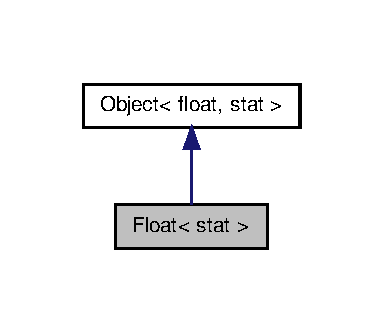
\includegraphics[width=184pt]{class_float__inherit__graph}
\end{center}
\end{figure}


Graphe de collaboration de Float$<$ stat $>$\-:\nopagebreak
\begin{figure}[H]
\begin{center}
\leavevmode
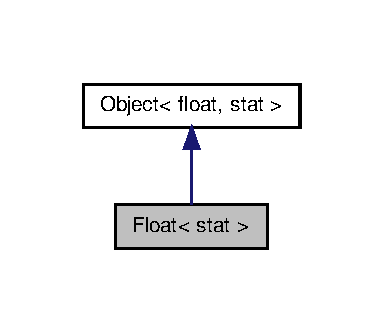
\includegraphics[width=184pt]{class_float__coll__graph}
\end{center}
\end{figure}
\subsection*{Fonctions membres publiques}
\begin{DoxyCompactItemize}
\item 
\hyperlink{class_float_af137dbc793f0678dda40b35b46d2c8c1}{Float} ()
\item 
\hyperlink{class_float_a1af3edf1b1def9e037aee6a23f7dd3fe}{Float} (const float \&i)
\item 
virtual \hyperlink{class_float_ac45409abc74786e686cf829c4876a0aa}{$\sim$\-Float} ()
\item 
\hyperlink{class_float}{Float} \hyperlink{class_float_a8a3c435dd4a8876e5f5b5e46017e7394}{operator+} (const float \&i)
\item 
\hyperlink{class_float}{Float} \hyperlink{class_float_a4c9b974c747319474ad78fa4904142fd}{operator+} (const \hyperlink{class_float}{Float} \&e)
\item 
\hyperlink{class_float}{Float} \hyperlink{class_float_a3f90a63ad65b9e64dcfd3d25bff63044}{operator-\/} (const float \&i)
\item 
\hyperlink{class_float}{Float} \hyperlink{class_float_ae7deb493a7109c8630c9efde48459324}{operator-\/} (const \hyperlink{class_float}{Float} \&e)
\item 
\hyperlink{class_float}{Float} \hyperlink{class_float_aeddcfb21e099ca1dca7bfb01b1b940da}{operator$\ast$} (const float \&i)
\item 
\hyperlink{class_float}{Float} \hyperlink{class_float_a7c419e58473a3999e3150f24c21751fc}{operator$\ast$} (const \hyperlink{class_float}{Float} \&e)
\item 
\hyperlink{class_float}{Float} \hyperlink{class_float_afa3921fc34b380a4585e20a871c62a04}{operator/} (const float \&i)
\item 
\hyperlink{class_float}{Float} \hyperlink{class_float_a7a3505f902424b8b28b951c3d8821092}{operator/} (const \hyperlink{class_float}{Float} \&e)
\item 
\hyperlink{class_float}{Float} \hyperlink{class_float_a6dd062495cb347e578eb1358bd148652}{operator\%} (const float \&i)
\item 
\hyperlink{class_float}{Float} \hyperlink{class_float_a3c147fcf9399759d332fa1cbd639a6bd}{operator\%} (const \hyperlink{class_float}{Float} \&e)
\item 
\hyperlink{class_float}{Float} \& \hyperlink{class_float_a48358fec8b2e99f931c5bf58974702e8}{operator++} ()
\item 
\hyperlink{class_float}{Float} \& \hyperlink{class_float_a898785de683a3f713e204bd215e955aa}{operator-\/-\/} ()
\item 
\hyperlink{class_float}{Float} \& \hyperlink{class_float_a186e649c71eade88e00550424cfa5d97}{operator+=} (const float \&i)
\item 
\hyperlink{class_float}{Float} \& \hyperlink{class_float_aa21413928861c3bcb4d7ab8716ed560b}{operator+=} (const \hyperlink{class_float}{Float} \&e)
\item 
\hyperlink{class_float}{Float} \& \hyperlink{class_float_a00dae468efad0ab93dadc37c5190e7ae}{operator-\/=} (const float \&i)
\item 
\hyperlink{class_float}{Float} \& \hyperlink{class_float_a644369b297eaefdae0ca276693ce7261}{operator-\/=} (const \hyperlink{class_float}{Float} \&e)
\item 
\hyperlink{class_float}{Float} \& \hyperlink{class_float_a249cb3e3648c43141b93aa24dc3bf1e6}{operator$\ast$=} (const float \&i)
\item 
\hyperlink{class_float}{Float} \& \hyperlink{class_float_a7c757c986315f93d481c56f7c9fb99f6}{operator$\ast$=} (const \hyperlink{class_float}{Float} \&e)
\item 
\hyperlink{class_float}{Float} \& \hyperlink{class_float_a0ed5beba2862fb7b045ba3c37fc79b84}{operator/=} (const float \&i)
\item 
\hyperlink{class_float}{Float} \& \hyperlink{class_float_a261f58fac8aef8d63b126dd3cf6e8033}{operator/=} (const \hyperlink{class_float}{Float} \&e)
\item 
\hyperlink{class_float}{Float} \& \hyperlink{class_float_aa1e0fdc5414ac89b911defd3037bfc51}{operator\%=} (const float \&i)
\item 
\hyperlink{class_float}{Float} \& \hyperlink{class_float_a5bf274605ae0174be0e34b79a4761e2d}{operator\%=} (const \hyperlink{class_float}{Float} \&e)
\end{DoxyCompactItemize}
\subsection*{Additional Inherited Members}


\subsection{Description détaillée}
\subsubsection*{template$<$Stat $\ast$ stat$>$class Float$<$ stat $>$}

La classe \hyperlink{class_float}{Float} répresente un modele de classe de type float et une réference vers une instance de statistique. La classe \hyperlink{class_float}{Float} hérite de la spécification de \hyperlink{class_object}{Object$<$float,stat$>$} 

\subsection{Documentation des constructeurs et destructeur}
\hypertarget{class_float_af137dbc793f0678dda40b35b46d2c8c1}{\index{Float@{Float}!Float@{Float}}
\index{Float@{Float}!Float@{Float}}
\subsubsection[{Float}]{\setlength{\rightskip}{0pt plus 5cm}template$<$Stat $\ast$ stat$>$ {\bf Float}$<$ stat $>$\-::{\bf Float} (
\begin{DoxyParamCaption}
{}
\end{DoxyParamCaption}
)\hspace{0.3cm}{\ttfamily [inline]}}}\label{class_float_af137dbc793f0678dda40b35b46d2c8c1}
Constructeur. Donne une valeur par défaut à un flotant. 
\begin{DoxyTemplParams}{Template Parameters}
{\em stat} & réference vers la statistiques en cours d'utilisation. \\
\hline
\end{DoxyTemplParams}
\hypertarget{class_float_a1af3edf1b1def9e037aee6a23f7dd3fe}{\index{Float@{Float}!Float@{Float}}
\index{Float@{Float}!Float@{Float}}
\subsubsection[{Float}]{\setlength{\rightskip}{0pt plus 5cm}template$<$Stat $\ast$ stat$>$ {\bf Float}$<$ stat $>$\-::{\bf Float} (
\begin{DoxyParamCaption}
\item[{const float \&}]{i}
\end{DoxyParamCaption}
)\hspace{0.3cm}{\ttfamily [inline]}}}\label{class_float_a1af3edf1b1def9e037aee6a23f7dd3fe}
Constructeur. Donne une réference vers un element de type O à cet objet. 
\begin{DoxyTemplParams}{Template Parameters}
{\em stat} & réference vers la statistiques en cours d'utilisation. \\
\hline
\end{DoxyTemplParams}

\begin{DoxyParams}{Paramètres}
{\em i} & réference vers un flotant. \\
\hline
\end{DoxyParams}
\hypertarget{class_float_ac45409abc74786e686cf829c4876a0aa}{\index{Float@{Float}!$\sim$\-Float@{$\sim$\-Float}}
\index{$\sim$\-Float@{$\sim$\-Float}!Float@{Float}}
\subsubsection[{$\sim$\-Float}]{\setlength{\rightskip}{0pt plus 5cm}template$<$Stat $\ast$ stat$>$ virtual {\bf Float}$<$ stat $>$\-::$\sim${\bf Float} (
\begin{DoxyParamCaption}
{}
\end{DoxyParamCaption}
)\hspace{0.3cm}{\ttfamily [inline]}, {\ttfamily [virtual]}}}\label{class_float_ac45409abc74786e686cf829c4876a0aa}
Destructeur Detruit l'objet de type \hyperlink{class_float}{Float} 

\subsection{Documentation des fonctions membres}
\hypertarget{class_float_a6dd062495cb347e578eb1358bd148652}{\index{Float@{Float}!operator\%@{operator\%}}
\index{operator\%@{operator\%}!Float@{Float}}
\subsubsection[{operator\%}]{\setlength{\rightskip}{0pt plus 5cm}template$<$Stat $\ast$ stat$>$ {\bf Float} {\bf Float}$<$ stat $>$\-::operator\% (
\begin{DoxyParamCaption}
\item[{const float \&}]{i}
\end{DoxyParamCaption}
)\hspace{0.3cm}{\ttfamily [inline]}}}\label{class_float_a6dd062495cb347e578eb1358bd148652}
Surcharge de l'operateur \% 
\begin{DoxyParams}{Paramètres}
{\em i} & un flotant. \\
\hline
\end{DoxyParams}
\hypertarget{class_float_a3c147fcf9399759d332fa1cbd639a6bd}{\index{Float@{Float}!operator\%@{operator\%}}
\index{operator\%@{operator\%}!Float@{Float}}
\subsubsection[{operator\%}]{\setlength{\rightskip}{0pt plus 5cm}template$<$Stat $\ast$ stat$>$ {\bf Float} {\bf Float}$<$ stat $>$\-::operator\% (
\begin{DoxyParamCaption}
\item[{const {\bf Float}$<$ stat $>$ \&}]{e}
\end{DoxyParamCaption}
)\hspace{0.3cm}{\ttfamily [inline]}}}\label{class_float_a3c147fcf9399759d332fa1cbd639a6bd}
Surcharge de l'operateur \% 
\begin{DoxyParams}{Paramètres}
{\em e} & un objet \hyperlink{class_float}{Float}. \\
\hline
\end{DoxyParams}
\hypertarget{class_float_aa1e0fdc5414ac89b911defd3037bfc51}{\index{Float@{Float}!operator\%=@{operator\%=}}
\index{operator\%=@{operator\%=}!Float@{Float}}
\subsubsection[{operator\%=}]{\setlength{\rightskip}{0pt plus 5cm}template$<$Stat $\ast$ stat$>$ {\bf Float}\& {\bf Float}$<$ stat $>$\-::operator\%= (
\begin{DoxyParamCaption}
\item[{const float \&}]{i}
\end{DoxyParamCaption}
)\hspace{0.3cm}{\ttfamily [inline]}}}\label{class_float_aa1e0fdc5414ac89b911defd3037bfc51}
Surcharge de l'operateur de réaffectation avec le modulo 
\begin{DoxyParams}{Paramètres}
{\em i} & un flotant. \\
\hline
\end{DoxyParams}
\hypertarget{class_float_a5bf274605ae0174be0e34b79a4761e2d}{\index{Float@{Float}!operator\%=@{operator\%=}}
\index{operator\%=@{operator\%=}!Float@{Float}}
\subsubsection[{operator\%=}]{\setlength{\rightskip}{0pt plus 5cm}template$<$Stat $\ast$ stat$>$ {\bf Float}\& {\bf Float}$<$ stat $>$\-::operator\%= (
\begin{DoxyParamCaption}
\item[{const {\bf Float}$<$ stat $>$ \&}]{e}
\end{DoxyParamCaption}
)\hspace{0.3cm}{\ttfamily [inline]}}}\label{class_float_a5bf274605ae0174be0e34b79a4761e2d}
Surcharge de l'operateur de réaffectation avec le modulo 
\begin{DoxyParams}{Paramètres}
{\em e} & un objet \hyperlink{class_float}{Float}. \\
\hline
\end{DoxyParams}
\hypertarget{class_float_aeddcfb21e099ca1dca7bfb01b1b940da}{\index{Float@{Float}!operator$\ast$@{operator$\ast$}}
\index{operator$\ast$@{operator$\ast$}!Float@{Float}}
\subsubsection[{operator$\ast$}]{\setlength{\rightskip}{0pt plus 5cm}template$<$Stat $\ast$ stat$>$ {\bf Float} {\bf Float}$<$ stat $>$\-::operator$\ast$ (
\begin{DoxyParamCaption}
\item[{const float \&}]{i}
\end{DoxyParamCaption}
)\hspace{0.3cm}{\ttfamily [inline]}}}\label{class_float_aeddcfb21e099ca1dca7bfb01b1b940da}
Surcharge de l'operateur $\ast$ 
\begin{DoxyParams}{Paramètres}
{\em i} & un flotant. \\
\hline
\end{DoxyParams}
\hypertarget{class_float_a7c419e58473a3999e3150f24c21751fc}{\index{Float@{Float}!operator$\ast$@{operator$\ast$}}
\index{operator$\ast$@{operator$\ast$}!Float@{Float}}
\subsubsection[{operator$\ast$}]{\setlength{\rightskip}{0pt plus 5cm}template$<$Stat $\ast$ stat$>$ {\bf Float} {\bf Float}$<$ stat $>$\-::operator$\ast$ (
\begin{DoxyParamCaption}
\item[{const {\bf Float}$<$ stat $>$ \&}]{e}
\end{DoxyParamCaption}
)\hspace{0.3cm}{\ttfamily [inline]}}}\label{class_float_a7c419e58473a3999e3150f24c21751fc}
Surcharge de l'operateur $\ast$ 
\begin{DoxyParams}{Paramètres}
{\em e} & un objet \hyperlink{class_float}{Float}. \\
\hline
\end{DoxyParams}
\hypertarget{class_float_a249cb3e3648c43141b93aa24dc3bf1e6}{\index{Float@{Float}!operator$\ast$=@{operator$\ast$=}}
\index{operator$\ast$=@{operator$\ast$=}!Float@{Float}}
\subsubsection[{operator$\ast$=}]{\setlength{\rightskip}{0pt plus 5cm}template$<$Stat $\ast$ stat$>$ {\bf Float}\& {\bf Float}$<$ stat $>$\-::operator$\ast$= (
\begin{DoxyParamCaption}
\item[{const float \&}]{i}
\end{DoxyParamCaption}
)\hspace{0.3cm}{\ttfamily [inline]}}}\label{class_float_a249cb3e3648c43141b93aa24dc3bf1e6}
Surcharge de l'operateur de réaffectation avec multiplication 
\begin{DoxyParams}{Paramètres}
{\em i} & un flotant. \\
\hline
\end{DoxyParams}
\hypertarget{class_float_a7c757c986315f93d481c56f7c9fb99f6}{\index{Float@{Float}!operator$\ast$=@{operator$\ast$=}}
\index{operator$\ast$=@{operator$\ast$=}!Float@{Float}}
\subsubsection[{operator$\ast$=}]{\setlength{\rightskip}{0pt plus 5cm}template$<$Stat $\ast$ stat$>$ {\bf Float}\& {\bf Float}$<$ stat $>$\-::operator$\ast$= (
\begin{DoxyParamCaption}
\item[{const {\bf Float}$<$ stat $>$ \&}]{e}
\end{DoxyParamCaption}
)\hspace{0.3cm}{\ttfamily [inline]}}}\label{class_float_a7c757c986315f93d481c56f7c9fb99f6}
Surcharge de l'operateur de réaffectation avec multiplication 
\begin{DoxyParams}{Paramètres}
{\em e} & un objet \hyperlink{class_float}{Float}. \\
\hline
\end{DoxyParams}
\hypertarget{class_float_a8a3c435dd4a8876e5f5b5e46017e7394}{\index{Float@{Float}!operator+@{operator+}}
\index{operator+@{operator+}!Float@{Float}}
\subsubsection[{operator+}]{\setlength{\rightskip}{0pt plus 5cm}template$<$Stat $\ast$ stat$>$ {\bf Float} {\bf Float}$<$ stat $>$\-::operator+ (
\begin{DoxyParamCaption}
\item[{const float \&}]{i}
\end{DoxyParamCaption}
)\hspace{0.3cm}{\ttfamily [inline]}}}\label{class_float_a8a3c435dd4a8876e5f5b5e46017e7394}
Surcharge de l'operateur + 
\begin{DoxyParams}{Paramètres}
{\em i} & un flotant. \\
\hline
\end{DoxyParams}
\hypertarget{class_float_a4c9b974c747319474ad78fa4904142fd}{\index{Float@{Float}!operator+@{operator+}}
\index{operator+@{operator+}!Float@{Float}}
\subsubsection[{operator+}]{\setlength{\rightskip}{0pt plus 5cm}template$<$Stat $\ast$ stat$>$ {\bf Float} {\bf Float}$<$ stat $>$\-::operator+ (
\begin{DoxyParamCaption}
\item[{const {\bf Float}$<$ stat $>$ \&}]{e}
\end{DoxyParamCaption}
)\hspace{0.3cm}{\ttfamily [inline]}}}\label{class_float_a4c9b974c747319474ad78fa4904142fd}
Surcharge de l'operateur + 
\begin{DoxyParams}{Paramètres}
{\em e} & un objet \hyperlink{class_float}{Float}. \\
\hline
\end{DoxyParams}
\hypertarget{class_float_a48358fec8b2e99f931c5bf58974702e8}{\index{Float@{Float}!operator++@{operator++}}
\index{operator++@{operator++}!Float@{Float}}
\subsubsection[{operator++}]{\setlength{\rightskip}{0pt plus 5cm}template$<$Stat $\ast$ stat$>$ {\bf Float}\& {\bf Float}$<$ stat $>$\-::operator++ (
\begin{DoxyParamCaption}
{}
\end{DoxyParamCaption}
)\hspace{0.3cm}{\ttfamily [inline]}}}\label{class_float_a48358fec8b2e99f931c5bf58974702e8}
Surcharge de l'operateur d'incrementation prefixe ++ \hypertarget{class_float_a186e649c71eade88e00550424cfa5d97}{\index{Float@{Float}!operator+=@{operator+=}}
\index{operator+=@{operator+=}!Float@{Float}}
\subsubsection[{operator+=}]{\setlength{\rightskip}{0pt plus 5cm}template$<$Stat $\ast$ stat$>$ {\bf Float}\& {\bf Float}$<$ stat $>$\-::operator+= (
\begin{DoxyParamCaption}
\item[{const float \&}]{i}
\end{DoxyParamCaption}
)\hspace{0.3cm}{\ttfamily [inline]}}}\label{class_float_a186e649c71eade88e00550424cfa5d97}
Surcharge de l'operateur de réaffecation avec incrementation 
\begin{DoxyParams}{Paramètres}
{\em i} & un flotant. \\
\hline
\end{DoxyParams}
\hypertarget{class_float_aa21413928861c3bcb4d7ab8716ed560b}{\index{Float@{Float}!operator+=@{operator+=}}
\index{operator+=@{operator+=}!Float@{Float}}
\subsubsection[{operator+=}]{\setlength{\rightskip}{0pt plus 5cm}template$<$Stat $\ast$ stat$>$ {\bf Float}\& {\bf Float}$<$ stat $>$\-::operator+= (
\begin{DoxyParamCaption}
\item[{const {\bf Float}$<$ stat $>$ \&}]{e}
\end{DoxyParamCaption}
)\hspace{0.3cm}{\ttfamily [inline]}}}\label{class_float_aa21413928861c3bcb4d7ab8716ed560b}
Surcharge de l'operateur de réaffecation avec incrementation 
\begin{DoxyParams}{Paramètres}
{\em e} & un objet \hyperlink{class_float}{Float}. \\
\hline
\end{DoxyParams}
\hypertarget{class_float_a3f90a63ad65b9e64dcfd3d25bff63044}{\index{Float@{Float}!operator-\/@{operator-\/}}
\index{operator-\/@{operator-\/}!Float@{Float}}
\subsubsection[{operator-\/}]{\setlength{\rightskip}{0pt plus 5cm}template$<$Stat $\ast$ stat$>$ {\bf Float} {\bf Float}$<$ stat $>$\-::operator-\/ (
\begin{DoxyParamCaption}
\item[{const float \&}]{i}
\end{DoxyParamCaption}
)\hspace{0.3cm}{\ttfamily [inline]}}}\label{class_float_a3f90a63ad65b9e64dcfd3d25bff63044}
Surcharge de l'operateur -\/ 
\begin{DoxyParams}{Paramètres}
{\em i} & un flotant. \\
\hline
\end{DoxyParams}
\hypertarget{class_float_ae7deb493a7109c8630c9efde48459324}{\index{Float@{Float}!operator-\/@{operator-\/}}
\index{operator-\/@{operator-\/}!Float@{Float}}
\subsubsection[{operator-\/}]{\setlength{\rightskip}{0pt plus 5cm}template$<$Stat $\ast$ stat$>$ {\bf Float} {\bf Float}$<$ stat $>$\-::operator-\/ (
\begin{DoxyParamCaption}
\item[{const {\bf Float}$<$ stat $>$ \&}]{e}
\end{DoxyParamCaption}
)\hspace{0.3cm}{\ttfamily [inline]}}}\label{class_float_ae7deb493a7109c8630c9efde48459324}
Surcharge de l'operateur -\/ 
\begin{DoxyParams}{Paramètres}
{\em e} & un objet \hyperlink{class_float}{Float}. \\
\hline
\end{DoxyParams}
\hypertarget{class_float_a898785de683a3f713e204bd215e955aa}{\index{Float@{Float}!operator-\/-\/@{operator-\/-\/}}
\index{operator-\/-\/@{operator-\/-\/}!Float@{Float}}
\subsubsection[{operator-\/-\/}]{\setlength{\rightskip}{0pt plus 5cm}template$<$Stat $\ast$ stat$>$ {\bf Float}\& {\bf Float}$<$ stat $>$\-::operator-\/-\/ (
\begin{DoxyParamCaption}
{}
\end{DoxyParamCaption}
)\hspace{0.3cm}{\ttfamily [inline]}}}\label{class_float_a898785de683a3f713e204bd215e955aa}
Surcharge de l'operateur de decrementation prefixe -- \hypertarget{class_float_a00dae468efad0ab93dadc37c5190e7ae}{\index{Float@{Float}!operator-\/=@{operator-\/=}}
\index{operator-\/=@{operator-\/=}!Float@{Float}}
\subsubsection[{operator-\/=}]{\setlength{\rightskip}{0pt plus 5cm}template$<$Stat $\ast$ stat$>$ {\bf Float}\& {\bf Float}$<$ stat $>$\-::operator-\/= (
\begin{DoxyParamCaption}
\item[{const float \&}]{i}
\end{DoxyParamCaption}
)\hspace{0.3cm}{\ttfamily [inline]}}}\label{class_float_a00dae468efad0ab93dadc37c5190e7ae}
Surcharge de l'operateur de réaffecation avec decrementation 
\begin{DoxyParams}{Paramètres}
{\em i} & un flotant. \\
\hline
\end{DoxyParams}
\hypertarget{class_float_a644369b297eaefdae0ca276693ce7261}{\index{Float@{Float}!operator-\/=@{operator-\/=}}
\index{operator-\/=@{operator-\/=}!Float@{Float}}
\subsubsection[{operator-\/=}]{\setlength{\rightskip}{0pt plus 5cm}template$<$Stat $\ast$ stat$>$ {\bf Float}\& {\bf Float}$<$ stat $>$\-::operator-\/= (
\begin{DoxyParamCaption}
\item[{const {\bf Float}$<$ stat $>$ \&}]{e}
\end{DoxyParamCaption}
)\hspace{0.3cm}{\ttfamily [inline]}}}\label{class_float_a644369b297eaefdae0ca276693ce7261}
Surcharge de l'operateur de réaffectation avec decrementation 
\begin{DoxyParams}{Paramètres}
{\em e} & un objet \hyperlink{class_float}{Float}. \\
\hline
\end{DoxyParams}
\hypertarget{class_float_afa3921fc34b380a4585e20a871c62a04}{\index{Float@{Float}!operator/@{operator/}}
\index{operator/@{operator/}!Float@{Float}}
\subsubsection[{operator/}]{\setlength{\rightskip}{0pt plus 5cm}template$<$Stat $\ast$ stat$>$ {\bf Float} {\bf Float}$<$ stat $>$\-::operator/ (
\begin{DoxyParamCaption}
\item[{const float \&}]{i}
\end{DoxyParamCaption}
)\hspace{0.3cm}{\ttfamily [inline]}}}\label{class_float_afa3921fc34b380a4585e20a871c62a04}
Surcharge de l'operateur / 
\begin{DoxyParams}{Paramètres}
{\em i} & un flotant. \\
\hline
\end{DoxyParams}
\hypertarget{class_float_a7a3505f902424b8b28b951c3d8821092}{\index{Float@{Float}!operator/@{operator/}}
\index{operator/@{operator/}!Float@{Float}}
\subsubsection[{operator/}]{\setlength{\rightskip}{0pt plus 5cm}template$<$Stat $\ast$ stat$>$ {\bf Float} {\bf Float}$<$ stat $>$\-::operator/ (
\begin{DoxyParamCaption}
\item[{const {\bf Float}$<$ stat $>$ \&}]{e}
\end{DoxyParamCaption}
)\hspace{0.3cm}{\ttfamily [inline]}}}\label{class_float_a7a3505f902424b8b28b951c3d8821092}
Surcharge de l'operateur / 
\begin{DoxyParams}{Paramètres}
{\em e} & un objet \hyperlink{class_float}{Float}. \\
\hline
\end{DoxyParams}
\hypertarget{class_float_a0ed5beba2862fb7b045ba3c37fc79b84}{\index{Float@{Float}!operator/=@{operator/=}}
\index{operator/=@{operator/=}!Float@{Float}}
\subsubsection[{operator/=}]{\setlength{\rightskip}{0pt plus 5cm}template$<$Stat $\ast$ stat$>$ {\bf Float}\& {\bf Float}$<$ stat $>$\-::operator/= (
\begin{DoxyParamCaption}
\item[{const float \&}]{i}
\end{DoxyParamCaption}
)\hspace{0.3cm}{\ttfamily [inline]}}}\label{class_float_a0ed5beba2862fb7b045ba3c37fc79b84}
Surcharge de l'operateur de réaffectation avec division 
\begin{DoxyParams}{Paramètres}
{\em i} & un flotant. \\
\hline
\end{DoxyParams}
\hypertarget{class_float_a261f58fac8aef8d63b126dd3cf6e8033}{\index{Float@{Float}!operator/=@{operator/=}}
\index{operator/=@{operator/=}!Float@{Float}}
\subsubsection[{operator/=}]{\setlength{\rightskip}{0pt plus 5cm}template$<$Stat $\ast$ stat$>$ {\bf Float}\& {\bf Float}$<$ stat $>$\-::operator/= (
\begin{DoxyParamCaption}
\item[{const {\bf Float}$<$ stat $>$ \&}]{e}
\end{DoxyParamCaption}
)\hspace{0.3cm}{\ttfamily [inline]}}}\label{class_float_a261f58fac8aef8d63b126dd3cf6e8033}
Surcharge de l'operateur de réaffecation avec division 
\begin{DoxyParams}{Paramètres}
{\em e} & un objet \hyperlink{class_float}{Float}. \\
\hline
\end{DoxyParams}


La documentation de cette classe a été générée à partir du fichier suivant \-:\begin{DoxyCompactItemize}
\item 
/home/ufr\-\_\-info/workspace/\-F\-W\-Algorithms/header/Float.\-hpp\end{DoxyCompactItemize}

\hypertarget{class_object}{\section{Référence du modèle de la classe Object$<$ O, stat $>$}
\label{class_object}\index{Object$<$ O, stat $>$@{Object$<$ O, stat $>$}}
}


{\ttfamily \#include $<$Object.\-hpp$>$}



Graphe de collaboration de Object$<$ O, stat $>$\-:\nopagebreak
\begin{figure}[H]
\begin{center}
\leavevmode
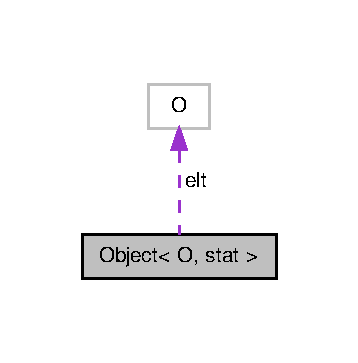
\includegraphics[width=172pt]{class_object__coll__graph}
\end{center}
\end{figure}
\subsection*{Fonctions membres publiques}
\begin{DoxyCompactItemize}
\item 
\hyperlink{class_object_a399244a9ba73c47997b5be3693cb497a}{Object} ()
\item 
\hyperlink{class_object_af5e2f97337e0536c71295cf2fc494534}{Object} (const O \&\hyperlink{class_object_ad6c327fe66540b59a513df29f755af4b}{elt})
\item 
virtual \hyperlink{class_object_a01a69e07247d7562664d90815e53b754}{$\sim$\-Object} ()
\item 
void \hyperlink{class_object_ab02a6925b233e2cecc5d05dcb63647b0}{operator=} (O \&\hyperlink{class_object_ad6c327fe66540b59a513df29f755af4b}{elt})
\item 
void \hyperlink{class_object_ab3871ba21ae0189d0c95f370d69bf3af}{operator=} (const \hyperlink{class_object}{Object} \&o)
\item 
bool \hyperlink{class_object_a1bff680d166704176bc6624e14b236fc}{operator$>$} (const O \&o)
\item 
bool \hyperlink{class_object_a285ff5c6899aa00a40caf7394adba387}{operator$>$} (const \hyperlink{class_object}{Object} \&o)
\item 
bool \hyperlink{class_object_a99b754624fdc54c737db3fb9cb629c66}{operator$<$} (const O \&o)
\item 
bool \hyperlink{class_object_ad56b7d529e52f15cb04e2379613cc7be}{operator$<$} (const \hyperlink{class_object}{Object} \&o)
\item 
bool \hyperlink{class_object_a9104e48bac2c6c9e01cef5ef5ce3f4e1}{operator$<$=} (const O \&o)
\item 
bool \hyperlink{class_object_a815b8628a0421c81d5ae55287d5252a4}{operator$<$=} (const \hyperlink{class_object}{Object} \&o)
\item 
bool \hyperlink{class_object_ab4abe75a80657646dbff7843d2d9b657}{operator$>$=} (const O \&o)
\item 
bool \hyperlink{class_object_a05637618e50fc65d1c0d7bf3cd9472dd}{operator$>$=} (const \hyperlink{class_object}{Object} \&o)
\item 
bool \hyperlink{class_object_a99010f4bd7aa5ca78c1eb2641e31f8f9}{operator==} (const O \&o)
\item 
bool \hyperlink{class_object_a266585d94b0deb105465fa7c89e8a1d9}{operator==} (const \hyperlink{class_object}{Object} \&o)
\item 
bool \hyperlink{class_object_a74a09ebb7325affab7a36722447ba3be}{operator!=} (const O \&o)
\item 
bool \hyperlink{class_object_ad9c2e8211d7e3822f88b56ef74a453e6}{operator!=} (const \hyperlink{class_object}{Object} \&o)
\item 
\hyperlink{class_object}{Object} \& \hyperlink{class_object_a0b5ab29ee535166da73a9663e40a404e}{operator$^\wedge$} (const O \&o)
\item 
\hyperlink{class_object}{Object} \& \hyperlink{class_object_a5e700ab1a5b8d7f03ab44e841fb0efcb}{operator$^\wedge$} (const \hyperlink{class_object}{Object} \&o)
\item 
\hyperlink{class_object}{Object} \& \hyperlink{class_object_a70555fefbc0832da61fda166b40aa6a8}{operator\&} (const O \&o)
\item 
\hyperlink{class_object}{Object} \& \hyperlink{class_object_a40ff14af9a98f948767b6a4c41ef215e}{operator\&} (const \hyperlink{class_object}{Object} \&o)
\item 
\hyperlink{class_object}{Object} \& \hyperlink{class_object_a10746acda9c977db58ce84678e027203}{operator$|$} (const O \&o)
\item 
\hyperlink{class_object}{Object} \& \hyperlink{class_object_a37e2268c6564f146ccac90d1a1a108e3}{operator$\sim$} ()
\end{DoxyCompactItemize}
\subsection*{Attributs protégés}
\begin{DoxyCompactItemize}
\item 
O \hyperlink{class_object_ad6c327fe66540b59a513df29f755af4b}{elt}
\end{DoxyCompactItemize}
\subsection*{Amis}
\begin{DoxyCompactItemize}
\item 
ostream \& \hyperlink{class_object_ab508b58bf37e341435dc0825e8274cb0}{operator$<$$<$} (ostream \&os, const \hyperlink{class_object}{Object} \&o)
\end{DoxyCompactItemize}


\subsection{Description détaillée}
\subsubsection*{template$<$class O, Stat $\ast$ stat$>$class Object$<$ O, stat $>$}

La classe \hyperlink{class_object}{Object} répresente un modele de classe de type O et une réference vers une instance de statistique. 

\subsection{Documentation des constructeurs et destructeur}
\hypertarget{class_object_a399244a9ba73c47997b5be3693cb497a}{\index{Object@{Object}!Object@{Object}}
\index{Object@{Object}!Object@{Object}}
\subsubsection[{Object}]{\setlength{\rightskip}{0pt plus 5cm}template$<$class O, Stat $\ast$ stat$>$ {\bf Object}$<$ O, stat $>$\-::{\bf Object} (
\begin{DoxyParamCaption}
{}
\end{DoxyParamCaption}
)\hspace{0.3cm}{\ttfamily [inline]}}}\label{class_object_a399244a9ba73c47997b5be3693cb497a}
Constructeur. Donne une valeur par défaut et un type O de cet objet. 
\begin{DoxyTemplParams}{Template Parameters}
{\em O} & type de l'objet à construire. \\
\hline
{\em stat} & réference vers la statistiques en cours d'utilisation. \\
\hline
\end{DoxyTemplParams}
\hypertarget{class_object_af5e2f97337e0536c71295cf2fc494534}{\index{Object@{Object}!Object@{Object}}
\index{Object@{Object}!Object@{Object}}
\subsubsection[{Object}]{\setlength{\rightskip}{0pt plus 5cm}template$<$class O, Stat $\ast$ stat$>$ {\bf Object}$<$ O, stat $>$\-::{\bf Object} (
\begin{DoxyParamCaption}
\item[{const O \&}]{elt}
\end{DoxyParamCaption}
)\hspace{0.3cm}{\ttfamily [inline]}}}\label{class_object_af5e2f97337e0536c71295cf2fc494534}
Constructeur. Donne une réference vers un element de type O à cet objet. 
\begin{DoxyTemplParams}{Template Parameters}
{\em O} & type de l'objet à construire. \\
\hline
{\em stat} & réference vers la statistiques en cours d'utilisation. \\
\hline
\end{DoxyTemplParams}

\begin{DoxyParams}{Paramètres}
{\em elt} & réference vers un element. \\
\hline
\end{DoxyParams}
\hypertarget{class_object_a01a69e07247d7562664d90815e53b754}{\index{Object@{Object}!$\sim$\-Object@{$\sim$\-Object}}
\index{$\sim$\-Object@{$\sim$\-Object}!Object@{Object}}
\subsubsection[{$\sim$\-Object}]{\setlength{\rightskip}{0pt plus 5cm}template$<$class O, Stat $\ast$ stat$>$ virtual {\bf Object}$<$ O, stat $>$\-::$\sim${\bf Object} (
\begin{DoxyParamCaption}
{}
\end{DoxyParamCaption}
)\hspace{0.3cm}{\ttfamily [inline]}, {\ttfamily [virtual]}}}\label{class_object_a01a69e07247d7562664d90815e53b754}
Destructeur. Detruit une object \hyperlink{class_object}{Object} 

\subsection{Documentation des fonctions membres}
\hypertarget{class_object_a74a09ebb7325affab7a36722447ba3be}{\index{Object@{Object}!operator!=@{operator!=}}
\index{operator!=@{operator!=}!Object@{Object}}
\subsubsection[{operator!=}]{\setlength{\rightskip}{0pt plus 5cm}template$<$class O, Stat $\ast$ stat$>$ bool {\bf Object}$<$ O, stat $>$\-::operator!= (
\begin{DoxyParamCaption}
\item[{const O \&}]{o}
\end{DoxyParamCaption}
)\hspace{0.3cm}{\ttfamily [inline]}}}\label{class_object_a74a09ebb7325affab7a36722447ba3be}
Surcharge de l'operateur de comparaison != 
\begin{DoxyParams}{Paramètres}
{\em o} & un element de type O. \\
\hline
\end{DoxyParams}
\hypertarget{class_object_ad9c2e8211d7e3822f88b56ef74a453e6}{\index{Object@{Object}!operator!=@{operator!=}}
\index{operator!=@{operator!=}!Object@{Object}}
\subsubsection[{operator!=}]{\setlength{\rightskip}{0pt plus 5cm}template$<$class O, Stat $\ast$ stat$>$ bool {\bf Object}$<$ O, stat $>$\-::operator!= (
\begin{DoxyParamCaption}
\item[{const {\bf Object}$<$ O, stat $>$ \&}]{o}
\end{DoxyParamCaption}
)\hspace{0.3cm}{\ttfamily [inline]}}}\label{class_object_ad9c2e8211d7e3822f88b56ef74a453e6}
Surcharge de l'operateur de comparaison != 
\begin{DoxyParams}{Paramètres}
{\em o} & un objet (\hyperlink{class_object}{Object}). \\
\hline
\end{DoxyParams}
\hypertarget{class_object_a70555fefbc0832da61fda166b40aa6a8}{\index{Object@{Object}!operator\&@{operator\&}}
\index{operator\&@{operator\&}!Object@{Object}}
\subsubsection[{operator\&}]{\setlength{\rightskip}{0pt plus 5cm}template$<$class O, Stat $\ast$ stat$>$ {\bf Object}\& {\bf Object}$<$ O, stat $>$\-::operator\& (
\begin{DoxyParamCaption}
\item[{const O \&}]{o}
\end{DoxyParamCaption}
)\hspace{0.3cm}{\ttfamily [inline]}}}\label{class_object_a70555fefbc0832da61fda166b40aa6a8}
Surcharge de l'operateur bit a bit \& 
\begin{DoxyParams}{Paramètres}
{\em o} & un element de type O. \\
\hline
\end{DoxyParams}
\hypertarget{class_object_a40ff14af9a98f948767b6a4c41ef215e}{\index{Object@{Object}!operator\&@{operator\&}}
\index{operator\&@{operator\&}!Object@{Object}}
\subsubsection[{operator\&}]{\setlength{\rightskip}{0pt plus 5cm}template$<$class O, Stat $\ast$ stat$>$ {\bf Object}\& {\bf Object}$<$ O, stat $>$\-::operator\& (
\begin{DoxyParamCaption}
\item[{const {\bf Object}$<$ O, stat $>$ \&}]{o}
\end{DoxyParamCaption}
)\hspace{0.3cm}{\ttfamily [inline]}}}\label{class_object_a40ff14af9a98f948767b6a4c41ef215e}
Surcharge de l'operateur bit a bit \& 
\begin{DoxyParams}{Paramètres}
{\em o} & un objet (\hyperlink{class_object}{Object}). \\
\hline
\end{DoxyParams}
\hypertarget{class_object_a99b754624fdc54c737db3fb9cb629c66}{\index{Object@{Object}!operator$<$@{operator$<$}}
\index{operator$<$@{operator$<$}!Object@{Object}}
\subsubsection[{operator$<$}]{\setlength{\rightskip}{0pt plus 5cm}template$<$class O, Stat $\ast$ stat$>$ bool {\bf Object}$<$ O, stat $>$\-::operator$<$ (
\begin{DoxyParamCaption}
\item[{const O \&}]{o}
\end{DoxyParamCaption}
)\hspace{0.3cm}{\ttfamily [inline]}}}\label{class_object_a99b754624fdc54c737db3fb9cb629c66}
Surcharge de l'operateur de comparaison $<$ 
\begin{DoxyParams}{Paramètres}
{\em o} & un element de type O. \\
\hline
\end{DoxyParams}
\hypertarget{class_object_ad56b7d529e52f15cb04e2379613cc7be}{\index{Object@{Object}!operator$<$@{operator$<$}}
\index{operator$<$@{operator$<$}!Object@{Object}}
\subsubsection[{operator$<$}]{\setlength{\rightskip}{0pt plus 5cm}template$<$class O, Stat $\ast$ stat$>$ bool {\bf Object}$<$ O, stat $>$\-::operator$<$ (
\begin{DoxyParamCaption}
\item[{const {\bf Object}$<$ O, stat $>$ \&}]{o}
\end{DoxyParamCaption}
)\hspace{0.3cm}{\ttfamily [inline]}}}\label{class_object_ad56b7d529e52f15cb04e2379613cc7be}
Surcharge de l'operateur de comparaison $<$ 
\begin{DoxyParams}{Paramètres}
{\em o} & un objet (\hyperlink{class_object}{Object}). \\
\hline
\end{DoxyParams}
\hypertarget{class_object_a9104e48bac2c6c9e01cef5ef5ce3f4e1}{\index{Object@{Object}!operator$<$=@{operator$<$=}}
\index{operator$<$=@{operator$<$=}!Object@{Object}}
\subsubsection[{operator$<$=}]{\setlength{\rightskip}{0pt plus 5cm}template$<$class O, Stat $\ast$ stat$>$ bool {\bf Object}$<$ O, stat $>$\-::operator$<$= (
\begin{DoxyParamCaption}
\item[{const O \&}]{o}
\end{DoxyParamCaption}
)\hspace{0.3cm}{\ttfamily [inline]}}}\label{class_object_a9104e48bac2c6c9e01cef5ef5ce3f4e1}
Surcharge de l'operateur de comparaison $<$= 
\begin{DoxyParams}{Paramètres}
{\em o} & un element de type O. \\
\hline
\end{DoxyParams}
\hypertarget{class_object_a815b8628a0421c81d5ae55287d5252a4}{\index{Object@{Object}!operator$<$=@{operator$<$=}}
\index{operator$<$=@{operator$<$=}!Object@{Object}}
\subsubsection[{operator$<$=}]{\setlength{\rightskip}{0pt plus 5cm}template$<$class O, Stat $\ast$ stat$>$ bool {\bf Object}$<$ O, stat $>$\-::operator$<$= (
\begin{DoxyParamCaption}
\item[{const {\bf Object}$<$ O, stat $>$ \&}]{o}
\end{DoxyParamCaption}
)\hspace{0.3cm}{\ttfamily [inline]}}}\label{class_object_a815b8628a0421c81d5ae55287d5252a4}
Surcharge de l'operateur de comparaison $<$= 
\begin{DoxyParams}{Paramètres}
{\em o} & un objet (\hyperlink{class_object}{Object}). \\
\hline
\end{DoxyParams}
\hypertarget{class_object_ab02a6925b233e2cecc5d05dcb63647b0}{\index{Object@{Object}!operator=@{operator=}}
\index{operator=@{operator=}!Object@{Object}}
\subsubsection[{operator=}]{\setlength{\rightskip}{0pt plus 5cm}template$<$class O, Stat $\ast$ stat$>$ void {\bf Object}$<$ O, stat $>$\-::operator= (
\begin{DoxyParamCaption}
\item[{O \&}]{elt}
\end{DoxyParamCaption}
)\hspace{0.3cm}{\ttfamily [inline]}}}\label{class_object_ab02a6925b233e2cecc5d05dcb63647b0}
Surcharge de l'operateur d'affectation = 
\begin{DoxyParams}{Paramètres}
{\em elt} & un element de type O. \\
\hline
\end{DoxyParams}
\hypertarget{class_object_ab3871ba21ae0189d0c95f370d69bf3af}{\index{Object@{Object}!operator=@{operator=}}
\index{operator=@{operator=}!Object@{Object}}
\subsubsection[{operator=}]{\setlength{\rightskip}{0pt plus 5cm}template$<$class O, Stat $\ast$ stat$>$ void {\bf Object}$<$ O, stat $>$\-::operator= (
\begin{DoxyParamCaption}
\item[{const {\bf Object}$<$ O, stat $>$ \&}]{o}
\end{DoxyParamCaption}
)\hspace{0.3cm}{\ttfamily [inline]}}}\label{class_object_ab3871ba21ae0189d0c95f370d69bf3af}
Surcharge de l'operateur d'affectation = 
\begin{DoxyParams}{Paramètres}
{\em o} & un objet (\hyperlink{class_object}{Object}). \\
\hline
\end{DoxyParams}
\hypertarget{class_object_a99010f4bd7aa5ca78c1eb2641e31f8f9}{\index{Object@{Object}!operator==@{operator==}}
\index{operator==@{operator==}!Object@{Object}}
\subsubsection[{operator==}]{\setlength{\rightskip}{0pt plus 5cm}template$<$class O, Stat $\ast$ stat$>$ bool {\bf Object}$<$ O, stat $>$\-::operator== (
\begin{DoxyParamCaption}
\item[{const O \&}]{o}
\end{DoxyParamCaption}
)\hspace{0.3cm}{\ttfamily [inline]}}}\label{class_object_a99010f4bd7aa5ca78c1eb2641e31f8f9}
Surcharge de l'operateur de comparaison == 
\begin{DoxyParams}{Paramètres}
{\em o} & un element de type O. \\
\hline
\end{DoxyParams}
\hypertarget{class_object_a266585d94b0deb105465fa7c89e8a1d9}{\index{Object@{Object}!operator==@{operator==}}
\index{operator==@{operator==}!Object@{Object}}
\subsubsection[{operator==}]{\setlength{\rightskip}{0pt plus 5cm}template$<$class O, Stat $\ast$ stat$>$ bool {\bf Object}$<$ O, stat $>$\-::operator== (
\begin{DoxyParamCaption}
\item[{const {\bf Object}$<$ O, stat $>$ \&}]{o}
\end{DoxyParamCaption}
)\hspace{0.3cm}{\ttfamily [inline]}}}\label{class_object_a266585d94b0deb105465fa7c89e8a1d9}
Surcharge de l'operateur de comparaison == 
\begin{DoxyParams}{Paramètres}
{\em o} & un objet (\hyperlink{class_object}{Object}). \\
\hline
\end{DoxyParams}
\hypertarget{class_object_a1bff680d166704176bc6624e14b236fc}{\index{Object@{Object}!operator$>$@{operator$>$}}
\index{operator$>$@{operator$>$}!Object@{Object}}
\subsubsection[{operator$>$}]{\setlength{\rightskip}{0pt plus 5cm}template$<$class O, Stat $\ast$ stat$>$ bool {\bf Object}$<$ O, stat $>$\-::operator$>$ (
\begin{DoxyParamCaption}
\item[{const O \&}]{o}
\end{DoxyParamCaption}
)\hspace{0.3cm}{\ttfamily [inline]}}}\label{class_object_a1bff680d166704176bc6624e14b236fc}
Surcharge de l'operateur de comparaison $>$ 
\begin{DoxyParams}{Paramètres}
{\em o} & un element de type O. \\
\hline
\end{DoxyParams}
\hypertarget{class_object_a285ff5c6899aa00a40caf7394adba387}{\index{Object@{Object}!operator$>$@{operator$>$}}
\index{operator$>$@{operator$>$}!Object@{Object}}
\subsubsection[{operator$>$}]{\setlength{\rightskip}{0pt plus 5cm}template$<$class O, Stat $\ast$ stat$>$ bool {\bf Object}$<$ O, stat $>$\-::operator$>$ (
\begin{DoxyParamCaption}
\item[{const {\bf Object}$<$ O, stat $>$ \&}]{o}
\end{DoxyParamCaption}
)\hspace{0.3cm}{\ttfamily [inline]}}}\label{class_object_a285ff5c6899aa00a40caf7394adba387}
Surcharge de l'operateur de comparaison $>$ 
\begin{DoxyParams}{Paramètres}
{\em o} & un objet (\hyperlink{class_object}{Object}). \\
\hline
\end{DoxyParams}
\hypertarget{class_object_ab4abe75a80657646dbff7843d2d9b657}{\index{Object@{Object}!operator$>$=@{operator$>$=}}
\index{operator$>$=@{operator$>$=}!Object@{Object}}
\subsubsection[{operator$>$=}]{\setlength{\rightskip}{0pt plus 5cm}template$<$class O, Stat $\ast$ stat$>$ bool {\bf Object}$<$ O, stat $>$\-::operator$>$= (
\begin{DoxyParamCaption}
\item[{const O \&}]{o}
\end{DoxyParamCaption}
)\hspace{0.3cm}{\ttfamily [inline]}}}\label{class_object_ab4abe75a80657646dbff7843d2d9b657}
Surcharge de l'operateur de comparaison $>$= 
\begin{DoxyParams}{Paramètres}
{\em o} & un element de type O. \\
\hline
\end{DoxyParams}
\hypertarget{class_object_a05637618e50fc65d1c0d7bf3cd9472dd}{\index{Object@{Object}!operator$>$=@{operator$>$=}}
\index{operator$>$=@{operator$>$=}!Object@{Object}}
\subsubsection[{operator$>$=}]{\setlength{\rightskip}{0pt plus 5cm}template$<$class O, Stat $\ast$ stat$>$ bool {\bf Object}$<$ O, stat $>$\-::operator$>$= (
\begin{DoxyParamCaption}
\item[{const {\bf Object}$<$ O, stat $>$ \&}]{o}
\end{DoxyParamCaption}
)\hspace{0.3cm}{\ttfamily [inline]}}}\label{class_object_a05637618e50fc65d1c0d7bf3cd9472dd}
Surcharge de l'operateur de comparaison $>$= 
\begin{DoxyParams}{Paramètres}
{\em o} & un objet (\hyperlink{class_object}{Object}). \\
\hline
\end{DoxyParams}
\hypertarget{class_object_a0b5ab29ee535166da73a9663e40a404e}{\index{Object@{Object}!operator$^\wedge$@{operator$^\wedge$}}
\index{operator$^\wedge$@{operator$^\wedge$}!Object@{Object}}
\subsubsection[{operator$^\wedge$}]{\setlength{\rightskip}{0pt plus 5cm}template$<$class O, Stat $\ast$ stat$>$ {\bf Object}\& {\bf Object}$<$ O, stat $>$\-::operator$^\wedge$ (
\begin{DoxyParamCaption}
\item[{const O \&}]{o}
\end{DoxyParamCaption}
)\hspace{0.3cm}{\ttfamily [inline]}}}\label{class_object_a0b5ab29ee535166da73a9663e40a404e}
Surcharge de l'operateur bit a bit $^\wedge$ 
\begin{DoxyParams}{Paramètres}
{\em o} & un element de type O. \\
\hline
\end{DoxyParams}
\hypertarget{class_object_a5e700ab1a5b8d7f03ab44e841fb0efcb}{\index{Object@{Object}!operator$^\wedge$@{operator$^\wedge$}}
\index{operator$^\wedge$@{operator$^\wedge$}!Object@{Object}}
\subsubsection[{operator$^\wedge$}]{\setlength{\rightskip}{0pt plus 5cm}template$<$class O, Stat $\ast$ stat$>$ {\bf Object}\& {\bf Object}$<$ O, stat $>$\-::operator$^\wedge$ (
\begin{DoxyParamCaption}
\item[{const {\bf Object}$<$ O, stat $>$ \&}]{o}
\end{DoxyParamCaption}
)\hspace{0.3cm}{\ttfamily [inline]}}}\label{class_object_a5e700ab1a5b8d7f03ab44e841fb0efcb}
Surcharge de l'operateur bit a bit $^\wedge$ 
\begin{DoxyParams}{Paramètres}
{\em o} & un objet (\hyperlink{class_object}{Object}). \\
\hline
\end{DoxyParams}
\hypertarget{class_object_a10746acda9c977db58ce84678e027203}{\index{Object@{Object}!operator$|$@{operator$|$}}
\index{operator$|$@{operator$|$}!Object@{Object}}
\subsubsection[{operator$|$}]{\setlength{\rightskip}{0pt plus 5cm}template$<$class O, Stat $\ast$ stat$>$ {\bf Object}\& {\bf Object}$<$ O, stat $>$\-::operator$|$ (
\begin{DoxyParamCaption}
\item[{const O \&}]{o}
\end{DoxyParamCaption}
)\hspace{0.3cm}{\ttfamily [inline]}}}\label{class_object_a10746acda9c977db58ce84678e027203}
Surcharge de l'operateur bit a bit $|$ 
\begin{DoxyParams}{Paramètres}
{\em o} & un element de type O. \\
\hline
\end{DoxyParams}
\hypertarget{class_object_a37e2268c6564f146ccac90d1a1a108e3}{\index{Object@{Object}!operator$\sim$@{operator$\sim$}}
\index{operator$\sim$@{operator$\sim$}!Object@{Object}}
\subsubsection[{operator$\sim$}]{\setlength{\rightskip}{0pt plus 5cm}template$<$class O, Stat $\ast$ stat$>$ {\bf Object}\& {\bf Object}$<$ O, stat $>$\-::operator$\sim$ (
\begin{DoxyParamCaption}
{}
\end{DoxyParamCaption}
)\hspace{0.3cm}{\ttfamily [inline]}}}\label{class_object_a37e2268c6564f146ccac90d1a1a108e3}
Surcharge de l'operateur bit a bit $\sim$ 

\subsection{Documentation des fonctions amies et associées}
\hypertarget{class_object_ab508b58bf37e341435dc0825e8274cb0}{\index{Object@{Object}!operator$<$$<$@{operator$<$$<$}}
\index{operator$<$$<$@{operator$<$$<$}!Object@{Object}}
\subsubsection[{operator$<$$<$}]{\setlength{\rightskip}{0pt plus 5cm}template$<$class O, Stat $\ast$ stat$>$ ostream\& operator$<$$<$ (
\begin{DoxyParamCaption}
\item[{ostream \&}]{os, }
\item[{const {\bf Object}$<$ O, stat $>$ \&}]{o}
\end{DoxyParamCaption}
)\hspace{0.3cm}{\ttfamily [friend]}}}\label{class_object_ab508b58bf37e341435dc0825e8274cb0}
Operateur de redirection du flux de sortie standard cout 
\begin{DoxyParams}{Paramètres}
{\em os} & flux de sortie standard \\
\hline
{\em o} & un objet \\
\hline
\end{DoxyParams}


\subsection{Documentation des données membres}
\hypertarget{class_object_ad6c327fe66540b59a513df29f755af4b}{\index{Object@{Object}!elt@{elt}}
\index{elt@{elt}!Object@{Object}}
\subsubsection[{elt}]{\setlength{\rightskip}{0pt plus 5cm}template$<$class O, Stat $\ast$ stat$>$ O {\bf Object}$<$ O, stat $>$\-::elt\hspace{0.3cm}{\ttfamily [protected]}}}\label{class_object_ad6c327fe66540b59a513df29f755af4b}
élement de type O. 

La documentation de cette classe a été générée à partir du fichier suivant \-:\begin{DoxyCompactItemize}
\item 
/home/ufr\-\_\-info/workspace/\-F\-W\-Algorithms/header/Object.\-hpp\end{DoxyCompactItemize}

\hypertarget{class_stat}{\section{Référence de la classe Stat}
\label{class_stat}\index{Stat@{Stat}}
}


{\ttfamily \#include $<$Stat.\-hpp$>$}

\subsection*{Fonctions membres publiques}
\begin{DoxyCompactItemize}
\item 
\hyperlink{class_stat_ae928e5dc2e02aa907902d4f3b369ab4a}{Stat} ()
\item 
virtual \hyperlink{class_stat_a160eb53b49050e1e0ccbc9b907618f0a}{$\sim$\-Stat} ()
\item 
void \hyperlink{class_stat_adde36e2e32b49973dd5305fe11fb5b1c}{incr\-Nb\-Tests} ()
\item 
void \hyperlink{class_stat_ae6f901344ac36750f4146ee093823122}{incr\-Nb\-Aff} ()
\item 
void \hyperlink{class_stat_a25ec11af23e836818eb78ef1715b4c5c}{incr\-Nb\-Op\-Ar} ()
\item 
void \hyperlink{class_stat_a6b4e1dc31e5d14d639a1d73b95c372f7}{time\-\_\-reset} ()
\item 
void \hyperlink{class_stat_aadb6e5b25d33840ea7c72e4badc53087}{show\-\_\-stats} ()
\item 
void \hyperlink{class_stat_a936652faec132143ebfd49dd324a049f}{print\-\_\-time} ()
\item 
void \hyperlink{class_stat_a406cc02790b5aa1e20c3c9bb29f25623}{print\-\_\-tests} ()
\item 
void \hyperlink{class_stat_a0c7005a7219c0ffa6e9bda7041eaa363}{print\-\_\-assignments} ()
\item 
void \hyperlink{class_stat_aad4baf34d7c7f18087eac414a349a2af}{print\-\_\-opar} ()
\end{DoxyCompactItemize}
\subsection*{Attributs protégés}
\begin{DoxyCompactItemize}
\item 
int \hyperlink{class_stat_a6f53f0a3c4000e2bd0d1d6b5d343781e}{nb\-Tests}
\item 
int \hyperlink{class_stat_a53bde9523b4dce5f474d05daeb9cdde7}{nb\-Aff}
\item 
int \hyperlink{class_stat_a619b6bf5dde16db7838ca1e00852f155}{nb\-Op\-Ar}
\item 
clock\-\_\-t \hyperlink{class_stat_a1ad6ee4f3626f9ba6fdb847244403939}{chrono}
\end{DoxyCompactItemize}


\subsection{Description détaillée}
La classe \hyperlink{class_stat}{Stat} répresente un objet de statistique qui va mesurer des operations effectuées par un certain algorithmes. 

\subsection{Documentation des constructeurs et destructeur}
\hypertarget{class_stat_ae928e5dc2e02aa907902d4f3b369ab4a}{\index{Stat@{Stat}!Stat@{Stat}}
\index{Stat@{Stat}!Stat@{Stat}}
\subsubsection[{Stat}]{\setlength{\rightskip}{0pt plus 5cm}Stat\-::\-Stat (
\begin{DoxyParamCaption}
{}
\end{DoxyParamCaption}
)\hspace{0.3cm}{\ttfamily [inline]}}}\label{class_stat_ae928e5dc2e02aa907902d4f3b369ab4a}
Constructeur. Initialise une instance de la class \hyperlink{class_stat}{Stat}. \hypertarget{class_stat_a160eb53b49050e1e0ccbc9b907618f0a}{\index{Stat@{Stat}!$\sim$\-Stat@{$\sim$\-Stat}}
\index{$\sim$\-Stat@{$\sim$\-Stat}!Stat@{Stat}}
\subsubsection[{$\sim$\-Stat}]{\setlength{\rightskip}{0pt plus 5cm}virtual Stat\-::$\sim$\-Stat (
\begin{DoxyParamCaption}
{}
\end{DoxyParamCaption}
)\hspace{0.3cm}{\ttfamily [inline]}, {\ttfamily [virtual]}}}\label{class_stat_a160eb53b49050e1e0ccbc9b907618f0a}
Desctructeur. Detruit l'instance de la class \hyperlink{class_stat}{Stat}. 

\subsection{Documentation des fonctions membres}
\hypertarget{class_stat_ae6f901344ac36750f4146ee093823122}{\index{Stat@{Stat}!incr\-Nb\-Aff@{incr\-Nb\-Aff}}
\index{incr\-Nb\-Aff@{incr\-Nb\-Aff}!Stat@{Stat}}
\subsubsection[{incr\-Nb\-Aff}]{\setlength{\rightskip}{0pt plus 5cm}void Stat\-::incr\-Nb\-Aff (
\begin{DoxyParamCaption}
{}
\end{DoxyParamCaption}
)\hspace{0.3cm}{\ttfamily [inline]}}}\label{class_stat_ae6f901344ac36750f4146ee093823122}
Incremente le nombre d'operation d'affectations \hypertarget{class_stat_a25ec11af23e836818eb78ef1715b4c5c}{\index{Stat@{Stat}!incr\-Nb\-Op\-Ar@{incr\-Nb\-Op\-Ar}}
\index{incr\-Nb\-Op\-Ar@{incr\-Nb\-Op\-Ar}!Stat@{Stat}}
\subsubsection[{incr\-Nb\-Op\-Ar}]{\setlength{\rightskip}{0pt plus 5cm}void Stat\-::incr\-Nb\-Op\-Ar (
\begin{DoxyParamCaption}
{}
\end{DoxyParamCaption}
)\hspace{0.3cm}{\ttfamily [inline]}}}\label{class_stat_a25ec11af23e836818eb78ef1715b4c5c}
Incremente le nombre d'operation arithmétiques \hypertarget{class_stat_adde36e2e32b49973dd5305fe11fb5b1c}{\index{Stat@{Stat}!incr\-Nb\-Tests@{incr\-Nb\-Tests}}
\index{incr\-Nb\-Tests@{incr\-Nb\-Tests}!Stat@{Stat}}
\subsubsection[{incr\-Nb\-Tests}]{\setlength{\rightskip}{0pt plus 5cm}void Stat\-::incr\-Nb\-Tests (
\begin{DoxyParamCaption}
{}
\end{DoxyParamCaption}
)\hspace{0.3cm}{\ttfamily [inline]}}}\label{class_stat_adde36e2e32b49973dd5305fe11fb5b1c}
Incremente le nombre d'operation de comparaisons \hypertarget{class_stat_a0c7005a7219c0ffa6e9bda7041eaa363}{\index{Stat@{Stat}!print\-\_\-assignments@{print\-\_\-assignments}}
\index{print\-\_\-assignments@{print\-\_\-assignments}!Stat@{Stat}}
\subsubsection[{print\-\_\-assignments}]{\setlength{\rightskip}{0pt plus 5cm}void Stat\-::print\-\_\-assignments (
\begin{DoxyParamCaption}
{}
\end{DoxyParamCaption}
)\hspace{0.3cm}{\ttfamily [inline]}}}\label{class_stat_a0c7005a7219c0ffa6e9bda7041eaa363}
Affiche le nombre d'affectations d'un algorithme \hypertarget{class_stat_aad4baf34d7c7f18087eac414a349a2af}{\index{Stat@{Stat}!print\-\_\-opar@{print\-\_\-opar}}
\index{print\-\_\-opar@{print\-\_\-opar}!Stat@{Stat}}
\subsubsection[{print\-\_\-opar}]{\setlength{\rightskip}{0pt plus 5cm}void Stat\-::print\-\_\-opar (
\begin{DoxyParamCaption}
{}
\end{DoxyParamCaption}
)\hspace{0.3cm}{\ttfamily [inline]}}}\label{class_stat_aad4baf34d7c7f18087eac414a349a2af}
Affiche le nombre d'operations arithmétiques d'un algorithme \hypertarget{class_stat_a406cc02790b5aa1e20c3c9bb29f25623}{\index{Stat@{Stat}!print\-\_\-tests@{print\-\_\-tests}}
\index{print\-\_\-tests@{print\-\_\-tests}!Stat@{Stat}}
\subsubsection[{print\-\_\-tests}]{\setlength{\rightskip}{0pt plus 5cm}void Stat\-::print\-\_\-tests (
\begin{DoxyParamCaption}
{}
\end{DoxyParamCaption}
)\hspace{0.3cm}{\ttfamily [inline]}}}\label{class_stat_a406cc02790b5aa1e20c3c9bb29f25623}
Affiche le nombre de comparaisons d'un algorithme \hypertarget{class_stat_a936652faec132143ebfd49dd324a049f}{\index{Stat@{Stat}!print\-\_\-time@{print\-\_\-time}}
\index{print\-\_\-time@{print\-\_\-time}!Stat@{Stat}}
\subsubsection[{print\-\_\-time}]{\setlength{\rightskip}{0pt plus 5cm}void Stat\-::print\-\_\-time (
\begin{DoxyParamCaption}
{}
\end{DoxyParamCaption}
)\hspace{0.3cm}{\ttfamily [inline]}}}\label{class_stat_a936652faec132143ebfd49dd324a049f}
Affiche le temps d'execution d'un algorithme associé à une statistiques Son utilisation s'attend à la réinitialisation du chrono \hypertarget{class_stat_aadb6e5b25d33840ea7c72e4badc53087}{\index{Stat@{Stat}!show\-\_\-stats@{show\-\_\-stats}}
\index{show\-\_\-stats@{show\-\_\-stats}!Stat@{Stat}}
\subsubsection[{show\-\_\-stats}]{\setlength{\rightskip}{0pt plus 5cm}void Stat\-::show\-\_\-stats (
\begin{DoxyParamCaption}
{}
\end{DoxyParamCaption}
)\hspace{0.3cm}{\ttfamily [inline]}}}\label{class_stat_aadb6e5b25d33840ea7c72e4badc53087}
Affiche tous les stats \hypertarget{class_stat_a6b4e1dc31e5d14d639a1d73b95c372f7}{\index{Stat@{Stat}!time\-\_\-reset@{time\-\_\-reset}}
\index{time\-\_\-reset@{time\-\_\-reset}!Stat@{Stat}}
\subsubsection[{time\-\_\-reset}]{\setlength{\rightskip}{0pt plus 5cm}void Stat\-::time\-\_\-reset (
\begin{DoxyParamCaption}
{}
\end{DoxyParamCaption}
)\hspace{0.3cm}{\ttfamily [inline]}}}\label{class_stat_a6b4e1dc31e5d14d639a1d73b95c372f7}
Reinitialise le chrono de stat 

\subsection{Documentation des données membres}
\hypertarget{class_stat_a1ad6ee4f3626f9ba6fdb847244403939}{\index{Stat@{Stat}!chrono@{chrono}}
\index{chrono@{chrono}!Stat@{Stat}}
\subsubsection[{chrono}]{\setlength{\rightskip}{0pt plus 5cm}clock\-\_\-t Stat\-::chrono\hspace{0.3cm}{\ttfamily [protected]}}}\label{class_stat_a1ad6ee4f3626f9ba6fdb847244403939}
Temps d'execution (version Beta) \hypertarget{class_stat_a53bde9523b4dce5f474d05daeb9cdde7}{\index{Stat@{Stat}!nb\-Aff@{nb\-Aff}}
\index{nb\-Aff@{nb\-Aff}!Stat@{Stat}}
\subsubsection[{nb\-Aff}]{\setlength{\rightskip}{0pt plus 5cm}int Stat\-::nb\-Aff\hspace{0.3cm}{\ttfamily [protected]}}}\label{class_stat_a53bde9523b4dce5f474d05daeb9cdde7}
Nombre d'operations d'affectations \hypertarget{class_stat_a619b6bf5dde16db7838ca1e00852f155}{\index{Stat@{Stat}!nb\-Op\-Ar@{nb\-Op\-Ar}}
\index{nb\-Op\-Ar@{nb\-Op\-Ar}!Stat@{Stat}}
\subsubsection[{nb\-Op\-Ar}]{\setlength{\rightskip}{0pt plus 5cm}int Stat\-::nb\-Op\-Ar\hspace{0.3cm}{\ttfamily [protected]}}}\label{class_stat_a619b6bf5dde16db7838ca1e00852f155}
Nombre d'operations arithmétiques \hypertarget{class_stat_a6f53f0a3c4000e2bd0d1d6b5d343781e}{\index{Stat@{Stat}!nb\-Tests@{nb\-Tests}}
\index{nb\-Tests@{nb\-Tests}!Stat@{Stat}}
\subsubsection[{nb\-Tests}]{\setlength{\rightskip}{0pt plus 5cm}int Stat\-::nb\-Tests\hspace{0.3cm}{\ttfamily [protected]}}}\label{class_stat_a6f53f0a3c4000e2bd0d1d6b5d343781e}
Nombre d'operations de comparaisons 

La documentation de cette classe a été générée à partir du fichier suivant \-:\begin{DoxyCompactItemize}
\item 
/home/ufr\-\_\-info/workspace/\-F\-W\-Algorithms/header/Stat.\-hpp\end{DoxyCompactItemize}

\hypertarget{class_string}{\section{Référence du modèle de la classe String$<$ stat $>$}
\label{class_string}\index{String$<$ stat $>$@{String$<$ stat $>$}}
}


{\ttfamily \#include $<$String.\-hpp$>$}



Graphe d'héritage de String$<$ stat $>$\-:\nopagebreak
\begin{figure}[H]
\begin{center}
\leavevmode
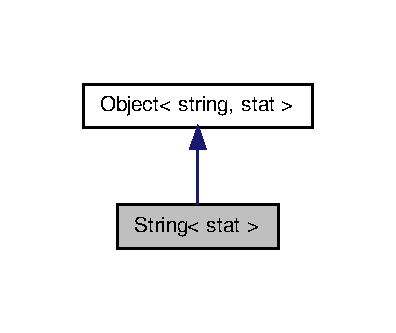
\includegraphics[width=190pt]{class_string__inherit__graph}
\end{center}
\end{figure}


Graphe de collaboration de String$<$ stat $>$\-:\nopagebreak
\begin{figure}[H]
\begin{center}
\leavevmode
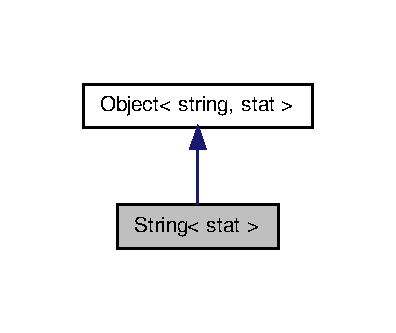
\includegraphics[width=190pt]{class_string__coll__graph}
\end{center}
\end{figure}
\subsection*{Fonctions membres publiques}
\begin{DoxyCompactItemize}
\item 
\hypertarget{class_string_abaa192ded1017246ee096d6a52c916a4}{{\bfseries String} (const string \&s)}\label{class_string_abaa192ded1017246ee096d6a52c916a4}

\end{DoxyCompactItemize}
\subsection*{Additional Inherited Members}


\subsection{Description détaillée}
\subsubsection*{template$<$Stat $\ast$ stat$>$class String$<$ stat $>$}

La classe \hyperlink{class_string}{String} répresente une classe de type string et une réference vers une instance de statistique. La classe \hyperlink{class_string}{String} hérite de la spécification de \hyperlink{class_object}{Object$<$string,stat$>$} 

La documentation de cette classe a été générée à partir du fichier suivant \-:\begin{DoxyCompactItemize}
\item 
/home/ufr\-\_\-info/workspace/\-F\-W\-Algorithms/header/String.\-hpp\end{DoxyCompactItemize}

\printindex
\end{document}
